\documentclass[11pt]{report}

\usepackage[pdftex, xdvi, dvips]{graphicx}
\usepackage{amsmath}
\usepackage{amssymb}
\usepackage{doublespace}
\usepackage{algorithm,algorithmic}
%\usepackage{epstopdf}
%\DeclareGraphicsRule{.tif}{png}{.png}{`convert #1 `basename #1 .tif`.png}

%\usepackage{amsmath}


\textwidth = 6.5 in
\textheight = 9 in
\oddsidemargin = 0.0 in
\evensidemargin = 0.0 in
\topmargin = 0.0 in
\headheight = 0.0 in
\headsep = 0.0 in
\parskip = 0.2in
\parindent = 0.0in



\newtheorem{theorem}{Theorem}
\newtheorem{acknowledgement}[theorem]{Acknowledgement}
%\newtheorem{algorithm}[theorem]{Algorithm}
\newtheorem{axiom}[theorem]{Axiom}
\newtheorem{case}[theorem]{Case}
\newtheorem{claim}[theorem]{Claim}
\newtheorem{conclusion}[theorem]{Conclusion}
\newtheorem{condition}[theorem]{Condition}
\newtheorem{conjecture}[theorem]{Conjecture}
\newtheorem{corollary}[theorem]{Corollary}
\newtheorem{criterion}[theorem]{Criterion}
\newtheorem{definition}[theorem]{Definition}
\newtheorem{example}[theorem]{Example}
\newtheorem{exercise}[theorem]{Exercise}
\newtheorem{lemma}[theorem]{Lemma}
\newtheorem{notation}[theorem]{Notation}
\newtheorem{problem}[theorem]{Problem}
\newtheorem{proposition}[theorem]{Proposition}
\newtheorem{remark}[theorem]{Remark}
\newtheorem{solution}[theorem]{Solution}
\newtheorem{summary}[theorem]{Summary}
\newenvironment{proof}[1][Proof]{\textbf{#1.} }{\ \rule{0.5em}{0.5em}}
%\input{tcilatex}


\title{Matrix Multiplication via Wavelets}
\author{Daniel Beatty}

\begin{document}

\maketitle 

%\frontmatter

\tableofcontents 

%\mainmatter



\chapter{Introduction}
Some overwhelming questions that drive computational science are how
fast can the answer be computed, how accurate is the answer, and how
stable is the method for obtaining the answer.  In this thesis, these
questions are applied to matrix multiplication. Of course there are already
conventional algorithms to compute matrix multiplication. This thesis
contributes a simple analysis of how the wavelet operator can be applied
to matrix multiplication.

The two most desired qualities in the computation of matrices are
sparseness and the condition number. Sparseness for a matrix states
that a good majority of the elements in such a matrix are zero.  The
condition number indicates how accurately an operation will be
performed on the system.  Wavelets contribute to numerical methods by
providing a stable preconditioning technique which produces a more
sparse and better conditioned than the original matrix.  Various forms
of the wavelet transform are key to applying wavelets as a
preconditioning tool.

Matrix multiplication has applications in simulations, computer
vision, and almost all areas of computational science.  Classic matrix
multiplication has a computational complexity of order $N^3$
operation, which makes it costly in the number of instructions that
are needed to carry out the operation. Faster matrix multiplication
techniques depend on the matrix being sparse to reduce the number
elements that need to be multiplied.  As shown in the results section,
there exists various levels of acceptable sparseness that are
generated by the wavelet transform.

For matrix multiplication, wavelets provide a preconditioning method
that transforms a dense matrix into a sparse one.  Thus sparse matrix
multiplication can be applied more effectively to general class of
matrices.  Wavelet preconditioning may or may not help for matrices
that are already sparse.

In this thesis, an overview is provided to define wavelets and how to
apply them.  This overview uses image processing to demonstrate the
qualities of a two-dimensional wavelet transform.  The next chapter
describes the wavelet matrix multiplication procedure. Chapter
\ref{chp:results} demonstrates matrix multiplication in the wavelet
domain and shows the results of different threshold levels on the
fidelity of the resulting product.  Finally, conclusions are
presented.



\chapter {Overview on Wavelets}
Wavelets evolved from atomic function theory where they were developed
as basic atoms or building blocks of all functions. This chapter
provides an overview of wavelets. This is done first by providing the
standard definitions and concepts of the wavelet basis function, the
wavelet transform and multiresolution representation. Then a numerical
example is utilized to demonstrate the concepts. The next section
details the numerical implementation of the wavelet transform. The
last section represents the 2D wavelet transform.

\section{The Wavelet Basis Function}

This section provides the basic properties of a wavelet function. It
first describes some general properties of functions. Then it presents
the translation and dilation properties which can be used to build an
entire bases. Finally, it presents the wavelet function itself.

\subsection{Function Properties}

There are a number of different properties that can be used to
classify functions. These include integrability, symmetry, compactness
and orthogonality. The properties will be introduced now and used in
the rest of the chapter.

A function, $f(\cdot)$, is {\it square integrable} if its $L_2$ norm is finite. This can be
expressed by
\[ 
f(x) \in L_2({\mathbb R}) \ \mbox{ if } \ \int\limits _{-\infty}^{\infty} \left|f(x)\right|^2 dx < \infty.
\]
A one-dimensional function is {\it symmetric} about the $y$-axis if 
\[
f(x) = f(-x)
\]
and it is {\it antisymmetric} if
\[
f(x) = -f(-x).
\]
The term symmetric is synonymous with ``even function.''  Likewise, antisymmetric is synonymous with ``odd functions.''

A set is considered {\it compact} in the $n$-dimensional real space,
${\mathbb R}^n$ if it is both closed and bounded. A function has {\it
compact support} if it is zero outside of a compact set. This implies that
there exists $n$-dimensional sphere, $S^n$, where 
\[
f(x) = 0 \qquad \forall x \not \in S^n.
\]

Orthogonality is another concept necessary for this thesis.  Two different basis functions are {\it orthogonal} if their inner product is zero.  The inner product of two functions, $f$ and $g$, can be represented by
\[
\left< f, g \right> = \int_{-\infty}^\infty f(x)g(x) \ dx.
\]
They are {\it orthonormal} if they are both orthogonal and have a norm of one.

\subsection {Translation and Dilation}

Translation shifts the basis function along the variable axis. The translation of a function, $f$, can be represented by $f_k$ where
\[
f_k(t) = f(t-k).
\]
Notice that translation does not alter the shape of the function, only the position of the function along the number space of $t$ \cite{translation}.

Dilation (also called contraction) transforms a one-dimensional function in width, and the output in height.   The dilation of a function, $f$, can be presented by $f_{j}$ where
\[
f_\alpha(t) = f(\alpha t).
\]
If $\alpha<1$ then the width of the function is increased. Otherwise it is decreased. 

Often, a scaling value is associated with the dilation operation.  An arbitrary form of this scaling is defined with $s$ as follows:
\[
f_s (t) = s f(t) 
\]
If $s>1$ then the height of the function is increased.   Likewise, when $s<1$ the height is decreased.  Often the scaling component is included in either translation, dilation or both.  In orthonormal-translation-dilation, there is a special case of notation as described next. 

These definitions can be combined into the translation-dilation representation upon dyadic intervals. A function $f$ can be expressed by a dilation of $j$ and a translation of $k$ through
\[
f_{j,k}(t) = 2^{j/2}f(2^jt-k) \qquad \forall j, k \in {\mathbb Z}.
\]
There is a special case for including the scaling factor of $2^{j/2}$.  The scaling value $2^{j/2}$ is applied to force a dyadic orthonormal condition.  
A function is said to have the orthonormal translation-dilation property when for two translation-dilations, $f_{j,k}$ and $f_{l,m}$, the result can be expressed by \cite{ChuiIntro}
\[
\left< f_{j,k} , f_{l,m} \right> = \delta_{j,l} \delta_{k,m}.
\]

\subsection {The Wavelet Basis Function}

The two mandatory properties of a wavelet basis function are:
\begin{itemize}
\item it must square integrable,   and
\item must have a zero average, i.e.:
\[
\int_{-\infty}^{+\infty}\psi(x) \ dx = 0.
\]
\end{itemize}
In addition, the class of orthogonal wavelet basis functions are restricted to satisfy
the orthonormal translation-dilation property. This restriction no longer applies to all wavelets by the lifting scheme % hasbeen removed through the lifting scheme 
\cite{fernandez96software}. An example
of a strict definition of a wavelet is given by Charles Chui \cite{ChuiIntro} (page 61):  
\begin{quote}
``A function $\psi \in L_2({\mathbb R})$ is called an orthonormal wavelet if the family $\{\psi_{j,k}\}$ defined 
\[ \psi_{j,k}(x)  = 2^{j/2} \psi (2 ^j x -k) \forall j,k \in {\mathbb Z} \]
is an orthonormal basis of $L_2({\mathbb R})$ where $\langle \psi _{j,k} , \psi_{l,m} \rangle = \delta _{j,l} \delta_{k,m}$,  $ \forall j,k,l,m\in {\mathbb Z}$ and every $ f\in L_2({\mathbb R})$ can be written as 
\[ f(x)= \sum\limits _{j,k = -\infty}^{\infty} c_{j,k} \psi _{j,k} (x)  \]
where the series convergences and is %of the series 
%\[ f(x) = \sum\limits _{j,k = -\infty}^{\infty}  c_{j,k} \psi _{j,k} (x)  \]
in $L_2({\mathbb R})$ such that 
\[ \lim\limits _{M_1, M_2, N_1 , N_2} || f - \sum\limits _{j=-M_2}^{N_2} \sum\limits _{k=-M_1}^{N_1} c_{j,k} \psi _{j,k} || = 0 \]
The simplest example of orthonormal wavelets is the Haar Transform.''
\end{quote}

There is more than one wavelet basis function. Additional classifications used include the symmetry and compactness \cite{jawerth94overview}. The Haar Wavelet Basis function actually fulfills the strictest definition of a wavelet basis function, and has additional properties.  The Haar Wavelet Basis Function has compact support.  It is also symmetric.  Furthermore, it has been stated by Walker\cite{walker}, Gregory Beylkin \cite{amsbeylkin,bvpbeylkin,fwtnal} and Chui \cite{ChuiIntro} that the Haar Wavelet Basis Function is the only wavelet basis function in $L_2({\mathbb R})$ that is orthogonal, compact, and symmetric.  The Haar wavelet basis function is defined below.
\begin{equation} \label{eqn:waveletbasis}
\psi(x) = \left\{
\begin{array}{cc}
1 & 0\le x < \frac{1}{2} \\
-1 & \frac{1}{2} \le x < 1 \\
0 & {otherwise}
\end{array}\right. 
\end{equation}


\section{The Wavelet Transform}

The wavelet transform is comprised of two parts, an average sample and
a difference sample. This is expressed by first looking at pairs of
wavelets and then looking at the actual representation.

\subsection {Wavelet Pairs: The Averaging Basis Function}

The Wavelet Basis Function section defined the Haar Wavelet Basis
Function defined the Haar Wavelet Basis function, in equation
\ref{eqn:waveletbasis}.  However, there exists a concept of a wavelet
pair.  These pairs exist as averaging and differencing basis.  The
wavelet basis function and differencing basis are synonymous.  The
averaging basis concept was derived from classic multi-resolution
which is described in section \ref{sec:multiresolution}.

This section only defines the wavelet basis pair in terms of a wavelet
averaging basis and shows an example with the Haar Averaging Basis
Function.  A wavelet pair is a set of two basis functions containing
one wavelet basis function and one averaging basis function which meet
the following criteria:
\begin{itemize}
\item both must be square integrable, 
\item both must satisfy the orthonormal dyadic translation-dilation property, and
\item the wavelet basis function must be orthogonal with the average basis function.
\end{itemize}
The simplest form of the averaging filter is the Haar Averaging
Filter, and it is a pair to the Haar Wavelet Basis Function.  Like the
Haar Wavelet Basis Function, the Haar Averaging Filter also satisfies
the dyadic-orthogonal translation property and is in $L_2({\mathbb R})$ The
mother \cite{walker,victor,ChuiIntro,tabor,graps} function for the Haar Averaging Filter is defined by
\[
\phi(x) =
\left\{\begin{array}{cc}1 & 0\le x < 1 \\0 &
{otherwise.}\end{array}\right.
\]

\subsection{Transform Representation}

This derivation uses the wavelet pair to define the wavelet transform.
Any wavelet transform uses a satisfactory wavelet pair to transform an
array into two halves which constitute the average filter sub-array
and the difference filtered sub-array.  This definition commonly
refers to the average filtered sub-array as the average terms and
difference terms, respectively.  The concatenated array of average and
difference terms constitutes a similar array to the original array,
and the same properties as similar vectors.  Also, for every wavelet
transform there is a straightforward method to restore the original
array from the wavelet transformed array called the inverse wavelet
transform.

One form of the wavelet transform is the integral wavelet transform
(IWT) described by Chui\cite{ChuiIntro}.  Another two are the discrete wavelet
transform (DWT) and the fast wavelet transform (FWT)\cite {walker, digital}.
  The convolution
wavelet transform (CWT) is a general form of the FWT.  In the case of
the CWT, any proper wavelet pairs can be used to generate corresponding
average and difference terms.  Application of the CWT is described in
section \ref{sec:implementation}.

Convolution of the wavelet pairs with an array form the starting point to the convolution wavelet transform.  The following constitute the steps of the CWT:
\begin{enumerate}
\item Convolute the original array $S$ with the wavelet pair.  The results of this are the average filtered array, $A$, and the difference filtered array, $D$.  
\item Selectively filter every other element of $A$ and $D$ into new arrays half the size of $S$.  The results map $A\to A'$ and $D\to D'$ respectively, where $A'$ and $D'$ are the selectively filtered average filter array, and selectively filtered difference filtered array, respectively.  
\item Concatenate $A'$ and $D'$ to form $W(S) = (A'|D')$, which is the wavelet transform of $S$.
\end{enumerate}

In the CWT used in this thesis, a modified version of the Haar Wavelet Basis Pair is used.   In particular, $\psi_{1,k}$ and its average basis function $\phi_{1,k}$ is the wavelet pair.  To assist the reader, this pair is defined for $x\in{\mathbb Z}$ in equations \ref{equ:haarphi1} and \ref{equ:haarpsi1}.  This basis pair is derived from the orthogonal dilation-translation equation for $j=1$, which is stated in equation \ref{equ:orthdiatrans1}.

\begin{equation}\label{equ:orthdiatrans1}
\psi_{j,k}(x)  = 2^{j/2} \psi (2 ^j x -k) \forall j,k \in {\mathbb Z} 
\end{equation}
%\begin{equation*}%\label{eqn:phi1}
\begin{eqnarray}
\label{equ:haarphi1}
\phi_{1,0}(x) = 2^{1/2} \phi (2 ^1 x ) =  \sqrt{\frac{1}{2}}
\left\{\begin{array}{cc}1 & x = 0\  {and} \ x = 1 \\0 & {otherwise} 
\end{array}\right.
\end{eqnarray}

\begin{eqnarray}\label{equ:haarpsi1}
\psi_{1,0}(x) = 2^{1/2} \psi (2 ^1 x ) = \sqrt{\frac{1}{2}}
 \left\{
\begin{array}{cc}
1 & x= 0 \\
-1 & x = 1 \\
0 & {otherwise}
\end{array}\right. 
\end{eqnarray}

%\end{equation}


\section{Multi-resolution Representation} \label{sec:multiresolution}

In one-dimensional, multi-resolution analysis provides a method to measure
averages, differences of the original array or signal and of the sub-arrays
generated in application of multi-resolution.  In this section,
techniques of multi-resolution are defined in terms of one-dimensional
wavelet transforms.  two-dimensional versions covered in section
\ref{sec:2Dwavelet}. Three methods for decomposing the signal are considered --- multiresolution analysis (MRA), multiresolution expansion (MRE) and the $\psi^n$ expansion.

\subsection{MRA} 

MRA schemes generates averaging estimates of some signal such that the
average representation is smaller than the original by some integer
amount.  MRA reapplies this averaging process until the process
produces a small enough size for the analysis being conducted.  MRA
may maintain estimate correction factors for the purpose of
translating an averaged array to the next larger average array to
recover that particular function.  The elements of average functions
are averaging terms.  Likewise, the elements of the estimate
correction factor function are called differencing terms.  To acquire
each estimate by wavelets, the wavelet averaging basis is used.  The
wavelet basis function happens to be the basis function for the
differencing function

There are simple ways to visualize this concept.  A classic one
dimensional form method is to consider a triangle.  In this triangle,
layers of functions are stacked up from the base to the apex.  The
original function is always placed on the bottom.  Subsequent average
terms are placed between the base and the apex.  For every level
between the apex and the base, there is an averaging method to map
that level to the adjacent level closer to the apex.  Also, there
exist a set of difference elements such that when the average is
expanded it can be mapped to the adjacent level toward the base.  The
apex has no adjacent level.  % to average to.  
The base has no difference
elements to map to a larger level.

The way to consider MRA with one-dimensional wavelet transforms is with a binary tree.  At the root of the tree, the entire original array is represented.  Two branches exist on this tree, the average and difference branch.  Each node in the tree represents a sub-array of the original array.   Branches are generated on a node if and only if a wavelet transform is performed on the node.  In case a wavelet transform is performed, both an average and difference branch are generated.  Otherwise the node is a leaf.  The following are rules for the one-dimensional wavelet transform binary tree in MRA:
\begin{itemize}
\item Transforms are only applied to leaves.
\item Transforms are only allowed on the root or average leaves.
\item If a node is not a leaf then a wavelet transformation has already been performed and is not permitted to be reapplied.
\item If the leaf is a difference term, then a transformation is not allowed.
\item The maximum height of this tree is $n = \lceil \log_2 \left|S\right| \rceil$ where $\left|S\right|$ is the cardinality of the signal $S$.
\end{itemize}   

\subsection{MRE}

MRE extends this idea by considering the difference leaves, also.  The rules for one-dimensional wavelet transform binary tree in MRA are as follows: 
%The maximum still represents a stopping condition.  In this case all elements within must be visited in order to perform this transformation.  Other stopping conditions may be imposed such as $L^2$ values,  
\begin{itemize}
\item Transforms are only applied to leaves.
\item If a node is not a leaf then a wavelet transformation has already been performed and is not permitted to be reapplied.
\item The maximum height of this tree is $n = \lceil \log_2 \left|S\right| \rceil$ where $\left|S\right|$ is the cardinality of the signal $S$.
\end{itemize}   

Like in MRA, there is an analogues to time and frequency signal representation.  Every sub-array represented at each node with in the wavelet transform binary tree represents activity in the time domain within a certain octave and note of frequencies.  That octave's frequency range is specified by its position within the array defined here:
\[
\left[
\frac{\pi x_1}{2 \cdot \left|S\right|} , \frac{\pi (x_2+1)}{2 \cdot \left|S\right|} 
\right]
\]
where $x_1$ is the starting index of the sub-array and $x_2$ is the ending index of the sub-array.

\subsection{$\psi^n$ Expansion}

There is another expansion similar to MRE which places its sections in a different arrangement.  This form is called the $\psi^n$ expansion.  It is a rather simple expansion of the wavelet transform.  Each resolution, reapplies the wavelet transform to the whole array again.  While it is simple to conceive and implement, the results are little more complicated to analyze.  A mapping procedure does exist for mapping the $\psi^n$ expansion to the MRE and vice versa.  

\section {Numerical Example}

To illustrate the concepts of the wavelet transform, four simple
numerical examples are provided.  First example shows the application of the CWT.  The second one utilities MRA and is
shown in Figure \ref{nummra}. The third one utilizes MRE and is
demonstrated in Figure \ref{nummre}.   In these examples,  the wavelet transform is applied to the source array $f$ defined in equation \ref{eqn:numexample}.  The CWT applied to source array $f$ is the Haar Convolution Wavelet Transform in the discrete domain.   More specifically, the Haar Convolution Wavelet Transform is defined for the Haar Wavelet Basis Pair  $\psi_{1,0}$ as in equation \ref {equ:haarpsi1} and $\phi_{1,0}$ in equation  \ref{equ:haarphi1}.  Lastly, the Haar Convolution Wavelet Transform in this case is the discrete form defined in terms of discrete convolution defined in equation \ref{eqn:convolution} in terms of the two operand arrays $f$ and $g$, and the result array $h$.
\begin{equation}
\label{eqn:numexample}
f(i) = \{5,5,5,3,4,6,8,5\} 
\end{equation}
\begin{equation}
\label{eqn:convolution}
 h_i = \langle f(l), g(-l + i) \rangle
\end{equation}
\subsection {Wavelet Transform Example}
This first example shows the CWT applied to the source array $f$.  
The first step is to acquire $A$ and $D$ defined:
\[A = S \ast \phi_1 \]
\[D = S \ast \psi_1 \] 
where $\phi_1$ and $\psi_1$ are a dilated Haar Wavelet Basis Pair defined in equations \ref{equ:haarphi1} and \ref{equ:haarpsi1}.   Each value $A_i$ and $D_i$ computed by these convolutions are simply the inner products of $\phi_1$ and $\psi_1$ translated by $i$ and are shown in equations \ref{haarphiinner} and \ref{haarpsiinner}.
\begin{equation}
\label {haarphiinner}
A_i = \langle S, \phi_{1,i} \rangle
\end{equation}
\begin{equation}
\label {haarpsiinner}
D_i = \langle S, \psi_{1,i} \rangle
\end{equation}
Each value of $A$ and $D$ are computed out in equations \ref{eqn:haaravecomp} and \ref{haardiffcomp}.  

\begin{eqnarray}
\label{eqn:haaravecomp}
S \ast \phi_1 =
\left(\begin{array}{ccc}
A_0  = & \langle S, \phi_{1, 0} \rangle = & \frac{5}{\sqrt{2}} \\
A_1  = & \langle S, \phi_{1, 1} \rangle = & 5\sqrt{2} \\
A_2  = & \langle S, \phi_{1, 2} \rangle = & 5\sqrt{2} \\
A_3  = & \langle S, \phi_{1, 3} \rangle = & 4\sqrt{2} \\
A_4  = & \langle S, \phi_{1, 4} \rangle = & \frac{7}{\sqrt{2}} \\
A_5  = & \langle S, \phi_{1, 5} \rangle = & 5\sqrt{2} \\
A_6  = & \langle S, \phi_{1, 6} \rangle = & 7\sqrt{2} \\
A_7  = & \langle S, \phi_{1, 7} \rangle = & \frac{13}{\sqrt{2} }
\end{array}\right)
\end{eqnarray}
\begin{eqnarray}
\label {haardiffcomp}
S \ast \psi_1 = \left(\begin{array}{ccc}
D_0 =& \langle S, \psi_{1, 0} \rangle=& \frac{5}{\sqrt{2}} \\
D_1=& \langle S, \psi_{1, 1} \rangle=& 0 \\
D_2=& \langle S, \psi_{1, 2} \rangle=& 0 \\
D_3=& \langle S, \psi_{1, 3} \rangle=& -{\sqrt{2}} \\
D_4=& \langle S, \psi_{1, 4} \rangle=& \sqrt{\frac{1}{2}} \\
D_5=& \langle S, \psi_{1, 5} \rangle=& \sqrt{2} \\
D_6=& \langle S, \psi_{1, 6} \rangle=& \sqrt{2} \\
D_7=& \langle S, \psi_{1, 7} \rangle=& \frac{-3}{\sqrt{2}}\end{array}\right)
\end {eqnarray}

Next, the selection filter removes all of the even indexed elements to produce $A'$ and $D'$.  Last,  $A'$ and $D'$ are concatenated to produce equation \ref{eqn:xforms}, which is the wavelet transform of $S$.  
\begin{equation*}
\label{eqn:xforms}
W(S(x)) = \{ 5\sqrt{2}, 4\sqrt{2}, 5\sqrt{2} , \frac{13}{\sqrt{2}}, 0, -\sqrt {2} , \sqrt{2}, -\frac{3}{\sqrt{2}} \}
\end{equation*}


\subsection {MRA Example}

MRA starts with the original array.  The wavelet transform is applied to the array.   After the first application of the wavelet transform, an average and difference array now exist.  This is shown in figure \ref{nummra} as the first two children in the wavelet binary tree.

\begin{figure}
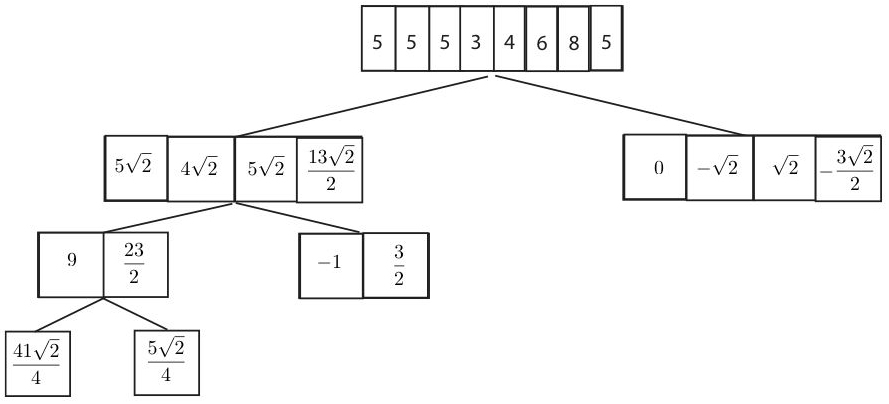
\includegraphics [width=6in]{mraexample2.jpg}
\caption{The Haar Transform performed a sample function show each step of the transform in multi-resolution analysis }
\label{nummra}
\end{figure}

For MRA, the analysis is continued on the average branch.  The difference branch is unchanged.  This procedure is repeated on the average branch.   The stopping point is determined by the size of array.  The finite limit, $n$, is 
\begin{equation} \label{eqn:treeheight} \displaystyle
n = \lceil\log_2 \left|S\right|\rceil
\end{equation}
where $\left|S\right|$ is the size of the array.

Once completed, the arrays are joined into an array which is the same
size as the original.  The energy is generally concentrated at the
beginning of the array.  Also, the energy of the array tends to be
ordered from strongest to weakest.  Terms representing change are kept
as pairs to each section.

Notice that the fine difference terms are left alone, and the dynamics
of the function in the time domain are accentuated.  Likewise the
lower frequency components are separated allowing a closer analysis in
both position and frequency.


\subsection {MRE Example}

Like MRA, MRE starts with an original array, and applies a wavelet transform to that array.  The decomposition is also represented by binary tree, with an average and difference branch.  The limit and height of the tree, $n$, remains the same as equation \ref{eqn:treeheight}.

\begin{figure}
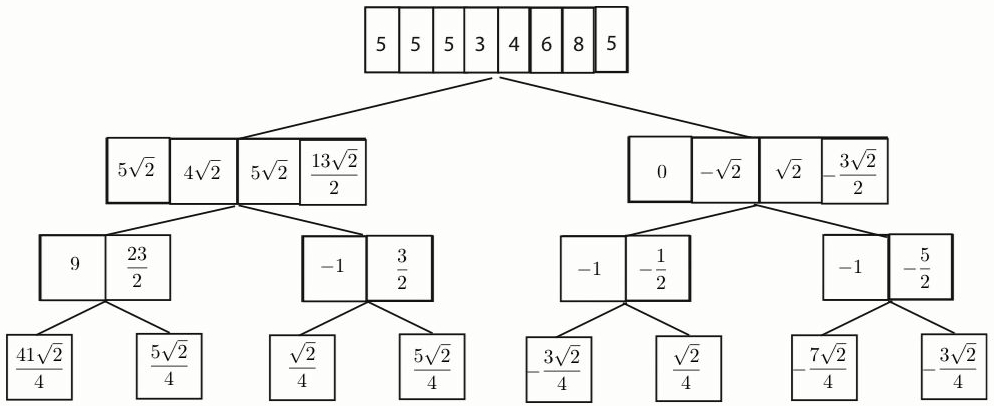
\includegraphics [width=6in]{numexample01_2.jpg}
\caption{The Haar Transform performed a sample function show each step of the transform in multi-resolution expansion }
\label{nummre}
\end{figure}

What is not the same is how the wavelet transform is reapplied.  In
addition to being applied on the average branch again, but the wavelet
transform is also applied to the difference branch also.  An example
is provided in Figure \ref{nummre}. The sub arrays are reinserted into
the array in order from the left branch to the right branch.

In the time and frequency analogues, each transformation filters the
array with high pass and low pass filter.  The frequency width of
these sub arrays is proportional to length of the original array.  The
center frequency is relative to the position of the sub-array within
the array.  The lowest frequency components are on the average side of
the array, and the highest frequency components are on the difference
section of the array.  One special case exists for arrays of length
$2^n$.  If the array is of length $2^n$, then the full MRE yields
entire frequency domain.  In case that the array is of odd size larger
than one, then the array must be padded and then normal decomposition
can continue.

  
\subsection {$\psi^n$ Expansion}
One other form of the multi-resolution expansion that can be used is almost trivial by its nature, $\psi^n$ expansion.  This particular form has the same branches as the MRE.  However, the sub arrays are place back in the array in a different order.    Figure \ref{numpsin} illustrates the difference in ordering from the $\psi^n$ form and the MRE form.    This form makes for a difficult analysis of time and frequency components, but contributes advantages linear operations.
\begin{figure}
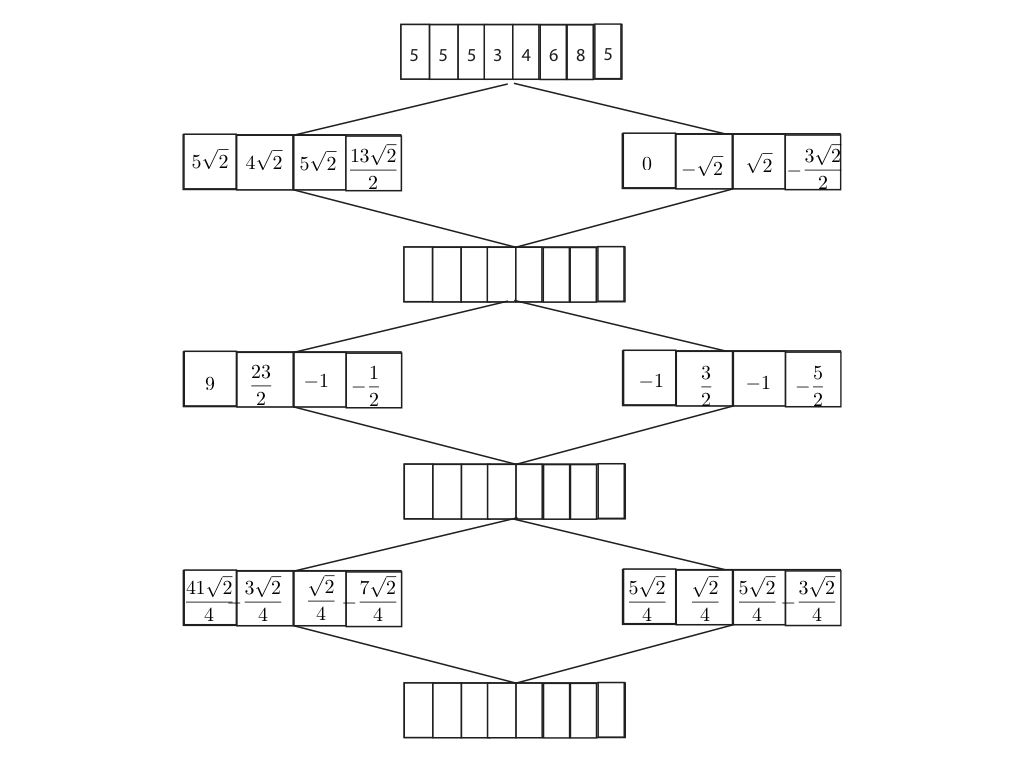
\includegraphics [width=6in]{psinexpansion.jpg}
\caption{The Haar Transform performed a sample function show each step of the transform in $\psi^n$ expansion }
\label{numpsin}
\end{figure}

\section{Implementation of the Wavelet Transform} \label{sec:implementation}

As stated before, the wavelet transform is defined in terms of average
and difference components. A signal is taken and transformed into the
two base objects.  Typically, the transform has the form $S\rightarrow
(A'|D')$ where $S$ is the original signal, $A$ is the average component,
$D$ is the difference component and $(A'|D')$ the signal $A'$
concatenated with $D'$.  This transformation can be modeled with the
convolution operator. Despite the decomposition of the signal into the
two components, the original signal can be reconstructed.

Many mathematicians such as Walker \cite{walker}, use a form that
eliminates half of the values. Thus a form can be defined which has
the same number of elements as the original.  The rules for choosing
the member elements are dependent on the wavelet filter choice. 
Another useful property of wavelets via convolution is the simplicity
of the operation. The general case works for all.  Such an algorithm
requires one nested loop as seen in Algorithm \ref{alg:convolution}.

\begin{algorithm}
\caption{Convolution of two signals $x(\cdot)$ and $h(\cdot)$.}
\label{alg:convolution}
\begin{algorithmic}
\STATE $y_i = 0$ $\forall i \in (0,M-1)$
\FOR{$i=0$ to $M-1$}
\FOR{$j=0$ to $N-1$}
\STATE $n=i-j$
\IF{$(0 \leq n < M)$}
\STATE$y(i) \  += \ x(j)\cdot h(n)$
\ENDIF
\ENDFOR
\ENDFOR
\end{algorithmic}
\end{algorithm}

This filter simply equates to the mathematical function
\[
y(k) = (x\ast h)(k) = \sum_{l}x(l)h(k-l)
\]
which is the convolution operation. It is obvious
that the operation is $O(NM)$ . For practical
use, the filter is made smaller than the actual signal being
analyzed. In some cases, the filter may be much smalled than the
signal. Filter size matters in extracting features from the original
signal.

To perform a wavelet transform via convolution, the signal is first
convolved with the average operator and then with the difference
operator.This can be represented by
\[
A = S \ast \phi 
\qquad \mbox{ and } \qquad
D = S \ast \psi.
\]
where $\phi$ is the mother wavelet and $\psi$ is the difference wavelet.

\section{The 2D Wavelet Transform} \label{sec:2Dwavelet}

For the 2D Wavelet Transform, it has to be determined how to represent
average and difference components. This can be done by creating one
average components and three difference component - vertical,
horizontal and diagonal. This can be used in a multiresolution fashion
to provide several levels of decomposition. 

A complete transform method returns a result matrix which is the same
size as the source matrix. The result contains the four
components. Each component resides on 4 corners of the matrix. Given a
matrix $B$, the transform is to yield the following form:
\[ 
B \Rightarrow 
\left(
\begin{array}{cc}
H & D \\ 
A & V
\end{array}
\right)
\]
where $A$ is the average component, $H$ is the horizontal component,
$V$ is the vertical component, and $D$ is the difference
component. There is another form which is also used as an example:
\[
B \Rightarrow 
\left(
\begin{array}{cc}
A & V \\ 
H & D
\end{array}
\right)
.\]
The first version is simple in concept, but provides a few more
possibilities for error and confusion.  Regardless of the case, the
four components have the following definitions:
\begin{enumerate}
\item Average component: produced by filtering the row vectors and the column vectors with the averaging filter.
\item Vertical Component:  produced by applying the average filter to the column vectors and the difference filter to the row vectors.
\item Horizontal component: produced by applying the average filter to the row vectors and the difference to the column vectors.
\item Diagonal component: produced by applying the difference filter to both the row and column vectors.  
\end{enumerate}

\subsection {Multi-Resolution in two-dimensions} 

Three methods are presented for decomposing 2D matrices --- 2D MRE, 2D
MRA and 2D $\psi^n$ Expansion. The first of these methods for matrices
is the 2D MRE.  In this form, the wavelet transform is applied
recursively to each of the sub-matrices.  The inverse of this MRE
applies the inverse wavelet transform is applied to the lowest level
adjacent sub-matrices.

The 2-D MRA is a special case of the 2-D MRE.  The application of the
wavelet transform is only applied to the average sub-matrix, only.
This method is also called wavelet pyramids.

The $\psi^n$ is rather more simple to implement, but is harder to
analyze.  In this case, the wavelet transform is simply reapplied to
the whole matrix.  The result of this method contains the same
elements as the 2-D MRE (wavelet transform full decomposition).
However, the arrangement of the elements is not the same.  This
arrangement will be used for matrix multiplication.

The method for visualizing 2D MRE and 2D MRA is similar to the
one-dimensional version.  Here a quadtree is used instead.  The four
branches represent the four sub-matrix types (average, vertical,
horizontal, and diagonal).  The rules for this tree is similar for the
1D wavelet transform binary tree.

The following are rules for the 2D wavelet transform quad tree in MRA.
\begin{itemize}
\item Transforms are only applied to leaves.
\item Transforms are only allowed on the root or average leaves.
\item If a node is not a leaf, then a wavelet transformation has already been performed and is not permitted to be reapplied.
\item If the leaf is a vertical, diagonal or horizontal term, then a transformation is not allowed.
\item The maximum height of this tree is 
$n = \min \left( \lceil N_r \rceil, \lceil N_c \rceil \right)$,
where $N_r$ is the number of rows in the matrix and $N_c$ is the number of columns in the matrix.
\end{itemize}   

MRE extends this idea by considering the difference leaves, also.  The rules for the 2D wavelet transform quad tree in MRA are below.
\begin{itemize}
\item Transforms are only applied to leaves.
\item If a node is not a leaf, then a wavelet transformation has already been performed and is not permitted to be reapplied.
\item The maximum height of this tree is 
$n = \min \left( \lceil N_r \rceil, \lceil N_c \rceil \right)$,
where $N_r$ is the number of rows in the matrix and $N_c$ is the number of columns in the matrix.
\end{itemize}   



%\subsection{Proof of Concept}
\subsection{Methods of Implementation}
Two methods of convolving a matrix are easily conceived.  First is to
use 1D wavelet.  The other is to apply the convolution scheme
straight to the matrix. Included in the wavelet experiment are both.
Realistically, both can and do achieve the same result.  However, the
direct method achieves speed advantages by the lack of overhead.  The
direct method only stores a temporary vector resident in memory.  Also,
there are two fewer transfers per row and column.

\subsubsection{1D to 2D Method}

Both rows 1D and 2D and columns 1D and 2D transform are performed
similarly.  The obvious difference is the indexing of rows and
columns.

\begin{algorithm}
\caption{Wavelet Row Transform}
\begin{algorithmic}
\REQUIRE Wavelet Transform, , and Wavelet Pair ($\psi$ and $\phi$)
\REQUIRE Matrix, $S \in {\mathbb R}^{N\times M}$
\FOR{$i = 0$ to $N-1$}
\STATE $R = S.getRow(i)$
\STATE $S.row(i) = \left[ R \ast \phi, R \ast \psi \right]$
\ENDFOR
\end{algorithmic}
\end{algorithm}

This principle of this algorithm is simple.  Only three intuitive steps are necessary per row or column.  Two of these steps are array transfers (row/column transfer to an array).  These arrays are fed into the 1D transforms.  

However, the 1D wavelet transform itself includes a series of memory allocation and deallocation operations.  Each memory call is at the minimum a system call.  

\subsubsection {Vector - Matrix Method}
The principle of this algorithm is more complicated.  All functionality, such as convolution, is built into the method.  There are fewer calls and passing of structures to external functions to compute the transform.  

This method has a few givens.  The source matrix, the Haar average filter, and the Haar difference filter are given arguments.  The result argument is the return argument.    The transform signals sub-function row transforms and column transforms to perform the work.  

The algorithm is as follows for the row transform (and is similar for the column transform):  

\begin{algorithm}
\caption{Wavelet Transform: Vector - Matrix Method: Row Transform }
\label{vmmethodrow}
\begin{algorithmic}
\REQUIRE  Wavelet Pair
\REQUIRE Temporary Vector $S$
\REQUIRE Matrix, $A \in {\mathbb R}^{M\times N}$
\FOR{$i = 0$ to $M$}
\STATE load $S$ from $A_i$ where $A_i$ is the row vector at row $i$
\STATE $S \stackrel{\psi_1}{\to} R$
\STATE Load $R$ into result matrix $\alpha$ at $\alpha_i$
\ENDFOR
\STATE Return $\alpha$
\end{algorithmic}
\end{algorithm}

\begin{algorithm}
\caption{Wavelet Transform: Vector - Matrix Method: Column Transform }
\label{vmmethodcol}
\begin{algorithmic}
\REQUIRE  Wavelet Pair
\REQUIRE Temporary Vector $S$
\REQUIRE Matrix, $A \in {\mathbb R}^{M\times N}$
\FOR{$j = 0$ to $N$}
\STATE load $S$ from $A_j$ where $A_i$ is the column vector at column $j$
\STATE $S \stackrel{\psi_1}{\to} R$
\STATE Load $R$ into result matrix $\alpha$ at $\alpha_j$
\ENDFOR
\STATE Return $\alpha$
\end{algorithmic}
\end{algorithm}

To perform a wavelet transform with this method, the driving wavelet transform method calls on of the wavelet transform methods and feeds the results into the other.  In the implementation used for this thesis, the row transform is called first,  then its results $\alpha$ are fed into the column transform as the column transforms $A$.  The results from the column transform are returned as the wavelet transform of the original matrix.  


\subsection{2-D MRA: Wavelet Pyramids}

This version of the wavelet transform (multiresolution) uses private members of the class $(hA, hD, xD/yD, xA/yA)$.  Both Haar filters are maintained this way.  Also both row and column transforms have average and difference myVector classes for temporary storage.   All of these members are allocated and destroyed by the wavelet transform method itself.   The simplified algorithm of the row transform is shown in Algorithm \ref{wpmethodrow}, and the column transform is shown in Algorithm \ref{wpmethodcol}.

\begin{algorithm}
\caption{Wavelet Transform: Wavelet Pyramid Method: Row Transform }
\label{wpmethodrow}
\begin{algorithmic}
\REQUIRE  Wavelet Pair $hA$ and $hD$ of length $w_l$
\REQUIRE Temporary Vector $S$
\REQUIRE Matrix, $A \in {\mathbb R}^{M\times N}$
\REQUIRE Limits of Rows and Columns to traverse: $M'$ and $N'$
%\REQUIRE Row index $i$
\REQUIRE Temporary vectors $xA$ and $xD$ for row Average vector and row Difference Vector.
\STATE Initialize vector $xA$ and $xD$
\FOR {$i = 0$ to $M'$}
\STATE Initialize $xA$ and $xD$
\FOR{$k = 0$ to $N'$}
\FOR {$l=0$ to $w_l$}
\STATE $n = k - l$
\IF {$n \in [0,N']$}
\STATE $xA_k = A_{i,n} \cdot hA_l$
\STATE $xD_k = A_{i,n} \cdot hD_l$
\ENDIF
\ENDFOR
\ENDFOR
\STATE Transfer to $\alpha$.  $\alpha_i  \leftarrow xA'|xD'$
\ENDFOR
\STATE Return $\alpha$
\end{algorithmic}
\end{algorithm}

\begin{algorithm}
\caption{Wavelet Transform: Wavelet Pyramid Method: Column Transform }
\label{wpmethodcol}
\begin{algorithmic}
\REQUIRE  Wavelet Pair $hA$ and $hD$ of length $w_l$
\REQUIRE Temporary Vector $S$
\REQUIRE Matrix, $A \in {\mathbb R}^{M\times N}$
\REQUIRE Limits of Rows and Columns to traverse: $M'$ and $N'$
%\REQUIRE Row index $i$
\REQUIRE Temporary vectors $yA$ and $yD$ for column Average vector and column Difference Vector.

\FOR {$j = 0$ to $N'$}
\STATE Initialize $yA$ and $yD$
\FOR{$k = 0$ to $M'$}
\FOR {$l=0$ to $w_l$}
\STATE $n = k - l$
\IF {$n \in [0,M']$}
\STATE $yA_k = A_{n,j} \cdot hA_l$
\STATE $yD_k = A_{n,j} \cdot hD_l$
\ENDIF
\ENDFOR
\ENDFOR
\STATE Transfer to $\alpha$.  $\alpha_j  \leftarrow yA'|yD'$
\ENDFOR
\STATE Return $\alpha$
\end{algorithmic}
\end{algorithm}

\begin{algorithm}
\caption{Wavelet Transform: Wavelet Pyramid Method: Driving Transform }
\label{wpmethod}
\begin{algorithmic}
\REQUIRE  Wavelet Pair $hA$ and $hD$ of length $w_l$
\REQUIRE Matrix $A$ of size $M\times N$
\REQUIRE Number of resolutions, $r$
\STATE Initialize matrix $\alpha$ to $M\times N$ and set equal to $A$
\STATE Initialize matrix $\beta$ to $M \times N$ and set equal to zero.
\FOR {$k = 0$ to $r$}
\STATE $M' = \frac{M}{2^k}$
\STATE $N' = \frac{N}{2^k}$
\STATE call row transform for matrix $\alpha$, with dimension limits $M'$ , $N'$ store in $\beta$
\STATE call column transform for matrix $\beta$, with dimension limits $M'$ , $N'$ store in $\alpha$
\ENDFOR
\STATE Return $\alpha$ as result
\end{algorithmic}
\end{algorithm}



Note: $A_i$ names the row vectors and $A_j$ names the column vectors, and $A_{i,j}$ is the element from the $i^{th}$ row and $j^{th}$ column.

The computational cost of this algorithm is $c \cdot C_\psi$  where $C_\psi$ is the cost of the wavelet transform at large, and $n$ is the number of resolutions performed.  The reason for this constant is that the size of the matrix being transformed shrinks by a factor of $2$ each time.  There may be additional overhead for the setup of the matrices, and transfer of matrix $S$ to $T$, which is $N^2$.  Since $C_\psi \propto O(N^2)$, and $c$ is based on $\log_2(N)$, then this a cost of another constant multiplied by $O(\sum\limits_{k=0}^{log_2(N)} \frac{1}{k^2}N^2))$.

\subsection {2-D MRE via Quad Tree}
There are two ways to implement the 2-D MRE and it depends on if other stopping conditions are desired.  The one stopping condition of size can be handled in a simple loop.  To enforce an energy limit stop, then a means to stop any further transforms on that branch must be used.   Two such means exist.   One way is to mark that branch and do so to its children.  Another way is to use a queue structure to designate nodes to be transform.  If the node represents a stopping condition, simply do not enter that node into the queue. 

In either case, the matrix information can be stored in this quad-tree.  Either by referencing position within the working matrix, or by storing a matrix in the node itself.  In this thesis, references were used for space efficiency.  However, the storage of the matrices in the nodes is just as valid.  Also a hybrid of only storing the final matrices in the leaves is acceptable as well.  

As stated, a straightforward loop can acquire the full decomposition.  The limit of the times required for is defined $v_l = 4^{r-1} $  where $r$ is the height of the quad-tree.  In this implementation, the quad tree is implemented in an array, and those properties are exploited in using a simple for loop to perform the 2-D MRE.
%    for ( index = r.id; index < length4; index++)
%    {
%        qtree->gotoNode(index);
%        qtree->getNode (temp);
%        selfRowWXform(temp);
%        selfColWXform(temp);
%        getSstats(temp);
\begin{algorithm}
\caption{Wavelet Transform: MRE Quad Tree Loop }
\label{mreqtloop}
\begin{algorithmic}
\REQUIRE Wavelet Transform, $\psi$, and Wavelet Pair
\REQUIRE Matrix, $S \in {\mathbb R}^{N\times M}$
\FOR{$i = 0$ to $v_l$}
\STATE draw $S$ from quad-tree at index $i$
\STATE $S \stackrel{\psi_r}{\to} T$
\STATE $T \stackrel{\psi_c}{\to} X$
\STATE Wavelet Split and Store $X$ in branch children.
\ENDFOR
\end{algorithmic}
\end{algorithm}

Note on Algorithm \ref{mreqtloop} that the Wavelet Split and Store operation splits the matrix $X$ into its four sub-matrices (average, horizontal, vertical, and diagonal) and stores them in their appropriate spot in the tree.  Thus every-time that $S$ is loaded a leaf branch of the tree is loaded to be transformed.  

The queue based 2-D MRE with a quad-tree is a bit more complicated.  The queue must be loaded with the root, then operation may be allowed to proceed.  The end condition is when the queue is empty.  Rules for loading the queue is must force the leaves on the last level to be ineligible for loading.    Otherwise, the loop will never stop and segmentation fault is likely to arise.  Energy rules and other arbitrary rules may also be imposed, but they are not as critical as the leaf limit rule.  For this example, refer to Algorithm \ref{wavemreloop}.
\begin{algorithm}
\caption {Wavelet Transform: MRE with queue controlled visits of the Quad Tree}
\label{wavemreloop}
\begin {algorithmic}
\REQUIRE Wavelet Transform, MRE, and wavelet pair ($\psi$ and $\phi$)
\REQUIRE Matrix $S$ 
\STATE {Insert root node representing the whole matrix in the queue.}
\WHILE {as long as queue is not empty} 
\STATE Get the next element from the queue, and load matrix $S$
\STATE $S \stackrel{\psi_r}{\to} T$
\STATE $T \stackrel{\psi_c}{\to} X$
\STATE Check $X$ for terminating conditions
\STATE if $X$ does not have a terminating condition store $X$'s four sections into the branch children of node $S$.  Store theses children nodes in the queue in order of average, vertical, horizontal, and difference.

\ENDWHILE
\end {algorithmic}
\end{algorithm}
The computational cost of this algorithm $n\cdot C_\psi$  where $C_\psi$ is the cost of the wavelet transform at large, and $n$ is the number of resolutions performed.  In some special cases, the cost may be slightly to significantly less if additional termination rules are applied.  The reduced size of the sub-matrices is canceled by quantity of sub-matrices to transform.  There may be additional overhead for the setup of the matrices.  Since $C_\psi \propto O(N^2)$, and $n$ is based on $\log_2(N)$ then this has a cost on the order of $N^2\log_2(N)$ also.  

%{
%    quadnode temp, temp2, a,v,h,d;
%    int ai, vi, hi, di;
%    queue->put (r);
%    int length = resolution;
%    int length4 = resolution / 4;
%    while (!queue->empty())
%    {
%        queue->get(temp);
%        if (qtree->gotoNode(temp.id) & (( temp.id ) < length4 ))
%            selfRowWXform(temp);
%            selfColWXform(temp);
%            getSstats (a);
%            getSstats (v);
%            getSstats (h);
%            getSstats (d);
%            ai = qtree->getA();
%            vi = qtree->getV();
%            hi = qtree->getH();
%            di = qtree->getD();
%            if ( ai < length4) {
%               qtree->getStats(S, ai);
%                qtree->getNode (ai, a);
%                queue->put(a);
%            }
%            if ( vi < length4) {
%                qtree->getStats(S, vi );
%                qtree->getNode (vi, v);
%                queue->put(v);
%            }
%            if ( hi < length4) {
%                qtree->getStats(S, hi );
%                qtree->getNode (hi, h);
%                queue->put(h);
%            }
%            if ( di <= length4) {
%                qtree->getStats(S, di );
%                qtree->getNode (di, d);
%                queue->put(d);



\subsection {2-D $\psi^n$ Implementation}
As stated the $\psi^n$ expansion is simpler to implement, but produces a matrix that is harder to analyze for features.  However, it is scientific merit since it is literally a wavelet transform of a wavelet transform.   Also, the limits imposed on the MRA and MRE for tree height are not required, but are rather a good idea.  A good practical limit would be for the resolution limit to be defined $n =\log_2 |S| -1$  where $|S|$ is the size of the the matrix S.  For this example, refer to Algorithm \ref{wavepsiloop}.
\begin{algorithm}
\caption {Wavelet Transform: MRE with queue controlled visits of the Quad Tree}
\label{wavepsiloop}
\begin {algorithmic}
\REQUIRE Wavelet Transform, MRE, and wavelet pair ($\psi$ and $\phi$)
\REQUIRE Matrix $S$ 
\STATE {Load $S$ into temporary matrix $T$}
\FOR {$i = 1$ to $n$}
\STATE {$T \stackrel{\psi_c}{\to} X$}
\STATE {$X \stackrel{\psi_r}{\to} T$}
\ENDFOR 
\STATE {return $T$ as the transformed matrix}

\end {algorithmic}
\end{algorithm}

The computational cost of this algorithm $n\cdot C_\psi$  where $C_\psi$ is the cost of the wavelet transform at large, and $n$ is the number of resolutions performed.  There may be additional overhead for the setup of the matrices, and transfer of matrix $S$ to $T$, which is $N^2$.  Since $C_\psi \propto O(N^2)$ then this has a cost on the order of $O(N^2\log_2(N))$.

%\section {Computational Cost}

%This should given after each algorithm.



%The cost of this algorithm is computed first for each row and each column.  This value is used to compute the cost of the matrix. The cost of computing the matrix is used to compute the cost of the multiresolution steps.   Per row the cost is $3K$, where $K$ is the number of columns.  Per column the cost is $3L$, where $L$ is the number of rows.  For the whole matrix, one resolution costs $6KL$ operations to compute the wavelet transform.    

%Per resolution with MRA, the rows and columns shrink by $2^i $ for each resolution, i, performed.  The limit of this cost equals $12KL$ operations.  If the values of $K$ and $L$ are relatively large, then it can be said that the order is $12N^2$ where $N$ is the worst case of the length or width of the matrix.    

%With either $psi^n$ expansion or MRE, the wavelet transform is reapplied to the whole matrix.  In the case of the $psi^n$ 

%Stopped at this point April 10, 2003



%\begin{thebibliography}{99}
%\bibitem {ChuiIntro} Charles Chui \textsl {An Introduction to Wavelets} published by Academic Press San Diego, CA 92101-4495 copyright 1992

%\bibitem{matrix01}Howard L. Resnikoff. and Raymond O. Wells, Jr. \textsl {Wavelet Analysis: The Scalable Structure of Information}  copyright Springer-Verlag New York, Inc.  New York, NY 10010, USA, 1998
%\bibitem{walker}James Walker \textsl {A Primer on Wavelets and Their Scientific Applications}
%copyright Chapman \& Hall/CRC : Boca Raton, FL, USA, 1999
%\bibitem{tabor}Gavin Tabor \textsl {Wavelets - The Idiots Guide} http://monet.me.ic.ac.uk/people/gavin/java/waveletDemos.html
%\bibitem {graps} Amara Graps \textsl {Introduction to Wavelets} http://www.amara.com/current/wavelet.html 

%\bibitem {appliedmethods} Singiresu S. Rao \textsl{Applied Numerical Methods for Engineers and Scientists}  published Prentice Hall Upper Saddle River, NJ 07458 copyright  2002
%\bibitem {numrecipies} William H. Press, Saul A. Teukolsky, William T. Vetterling, and Brian P. Flannery 

%\textsl {Numerical Methods in C}
%Published by the Press Syndicate of the University of Cambridge The Pitt Building, Trumpington Street, Cambridge CB2 1RP%40 West 20th Street, New York, NY 10011-4211, USA
%Copyright Cambridge University Press 1988, 1992

%\bibitem {bvpbeylkin}  G. Beylkin \textsl{On wavelet-based algorithms for solving differential equations}

%\bibitem {amsbeylkin}  G. Beylkin \textsl{Wavelets and Fast Numerical Algorithms}

%\bibitem {fwtnal} G. Beylkin, R. Coifman, and V. Rokhlin \textsl {Fast Wavelet Transforms and Numerical Algorithms I, Article in Communications on pure and applied mathematics} copyright 1991 Wiley, New York

%\bibitem {mwabeylkin}  G. Beylkin, D. Gines and L. Vozovoi \textsl{Adaptive Solution of Partial Differential Equations in Multiwavelet Bases }

%\bibitem {PDEfSE} Stanly J. Farlow \textsl{Partial Differential Equations for Scientists and Engineers} copywrite 1993 Dover Publications, Inc Mineola, N.Y. 11501

%\bibitem {spiegel} Murray R. Spiegel, \textsl { Theory and Problems of Advanced Mathematics for Engineers and Scientist} copy-write 1996 McGraw-Hill 

%\bibitem {tools} Stephane Jaffard, Yves Meyer, and Robert D. Ryan \textsl {Wavelets: Tools for Science and Technology} copyright 2001 by the Society for Industrial and Applied Mathematics Philadelphia, PA 19104-2688

%\bibitem {victor} Mladen Victor Wickerhauser \textsl {Adapted Wavelet Analysis from Theory to Software} copyright 2001 by the Society for Industrial and Applied Mathematics Philadelphia, PA 19104-2688

%\bibitem En-Bing Lin and Zhengchu Xiao \textsl {Multiwavelet Solutions for the Dirichlet Problem} Department of Mathematics, University of Toledo; Toledo, OH 43606, USA

%\bibitem Tian-Xiao He \textsl {Wavelet Analysis and Multiresolution Methods (Lecture Notes in Pure and Applied Mathematics} published Marcel Dekker, Inc.  New York, NY 10016 copyright 2000

%\bibitem {ChuiIntro} Charles Chui \textsl {An Introduction to Wavelets} published by Academic Press San Diego, CA 92101-4495 copyright 1992


%\end{thebibliography}

% \end{document}

 


\chapter{Image Processing Example of Wavelets}
This chapter is for showing graphically examples of the one-dimensional and two dimensional wavelet transform.  For one dimensional wavelet transform a simple sinusoid signal is used as the source input to measure correctness of the implementation.   Likewise, a simple pictorial image is used as the test input to show correctness of these implementations of the two dimensional wavelet transform.  

\section{Results --- 1D Wavelet Transform}

Testing of the 1D wavelet was performed on a sinusoidal wave form of 128 elements:
\begin{equation}\label{sinusoid}
y(n) = 10 \sin \left({n \over 128}\right) 
	- 5 \sin \left({n \over 64}\right) 
	+ 2 \sin \left({3 n \over 128}\right)
	- \sin \left({n \over 32}\right).
\end{equation}
This function  is the input function used for the one-dimensional implementations and is shown graphically in Figure \ref{sample}. The first test of the 1D transform used the even elements of both convolutions to generate the wavelet transform.  These even elements came from the over-complete form and naturally allow the potential to have complete information.  However, in doing so, a fundamental flaw appears.

\begin{figure}
\begin{center}\includegraphics [width=4in]{sample.jpg} \end{center}
\caption{Sample function.  The $x$-axis is the array index (index $n$).  The $y$ value is simple -- the value $y(n)$. }
\label{sample}
\end{figure}

In order to evaluate the effectiveness of the wavelet transform three
tests have been devised.  First, energy equivalence is used to
determine how much energy is retained in the transform from the
original.  The general shape is used on a the first resolution to test
if the average signal has the same general shape as the original.
Lastly, the inverse transform is used to recover the original signal.
A comparison is made between the original and the recovered signal.

After one resolution, the transformed signal has the same energy as
the original.  This is good since it allows the original to be
recovered from the transform.  Also, the average component of the
transform has the same shape as the original, which is good.  However,
the recovered signal is missing the last element.  Refer to Figure
\ref{recoverEven}. The secret is in which elements are used from the
over-complete to make the complete.  The over-complete form is defined
from the average and difference components which are simply the result
of convolution.

\begin{figure}
\begin{center}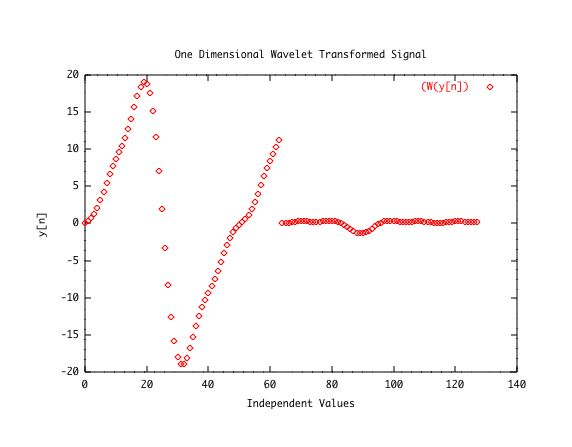
\includegraphics [width=6in]{haar1d.jpg} \end{center}
\caption{\label{wavelet_sample}
Signal after the wavelet transformation.}	
\end{figure}


The convolution means is at the heart of the issue.  The convolution operator in this case starts with the first element of the filter against the first element of the signal.  In the simple Haar Wavelet case, there is a transformation pairing
\[
(S_i , S_{i-1}) \rightarrow A_i, \mbox{ and } (S_i , S_{i-1}) \rightarrow D_i .
\]
In this pairing with zero indexed signals, the odd indexed elements from the over-complete must be used to have all elements of the original accounted for.   

Also this produces a functional difference between wavelet inverse transform for odd and even versions.  The difference is slight; however, the last element is lost in the even indexed form.  
\begin{eqnarray*}
\mbox{Odd: } \qquad R_{2i} =(A_i - D_i ) \sqrt{1/2}, &\qquad& R_{2i+1}=(A_i + D_i ) \sqrt{1/2} \\
\mbox{Even: } \qquad R_{2i} =(A_i + D_i ) \sqrt{1/2}, &\qquad& R_{2i-1}=(A_i - D_i ) \sqrt{1/2} 
\end{eqnarray*}


%The even split  and analysis of this transform.  
\begin{figure}
\begin{center}\includegraphics [width=6in]{recoveredEven.jpg} \end{center}
\caption{Recovered function.  The $x$-axis is the array index (index n).  The $y$ value is simply the value $y(n)$.  The function was recovered from an even indexed wavelet transform. }
\label{recoverEven}
\end{figure}

 
\begin{figure}
\begin{center}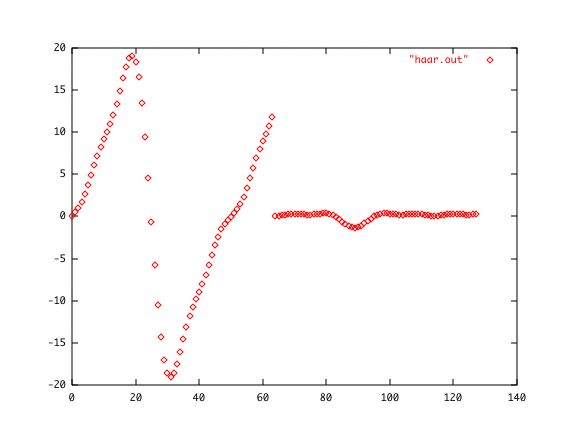
\includegraphics [width=6in]{recovered.jpg} \end{center}
\caption{Recovered function.  The x-axis is the array index (index n).  The y value is simply the value y[n].  The function was recovered from an odd indexed wavelet transform. }
\label{recoverOdd}
\end{figure}

An odd indexed wavelet transform yields the same energy.  However, all of the values are accounted for.  Refer to Figure \ref{recoverOdd}.  

\section {Results: 2D Wavelet Transform }
A simple room picture shows the difference that correct indexing produces in the wavelet transform and its inverse. The 1D to 2D method shows the incorrectly indexed case.  A correctly indexed version is shown in the vector-matrix method.  

The 1D to 2D implementation has a serious issue with memory leak errors.  Memory is allocated and deallocated quickly, and on some platforms shows up as an error.   Some platforms are not forgiving of this error and will force the program to terminate (Macintosh OSX 10.2, using gcc 3.1).    On other platforms, the error is tolerated and performance is degraded (IRIX, SGI Octane2 using gcc 2.9).   An example image of 720 x 486 required nearly 10 minutes to compute the wavelet transform by this method on an SGI Octane2.  However, it does eventually return a correct result.  

The matrix-vector method also yields the correct result.  However, there is less memory overhead in this method as compared to the 1D to 2D method.  As a result, both the row wavelet transform and column wavelet transforms are performed more quickly, with fewer memory transfers and allocations.  Obviously, this also allows for the operation to be conducted almost entirely in cache memory on both the SGI Octane2 and Macintosh G4 based machines.  A Macintosh G3 based machine still requires main memory at a minimum to execute the same operation.% which yields a slower performance.  

A correct result must also be matched to a correct inverse method.  The indexing order matters.  The inverse transform method is a forward inverse transform method.  In the case of 1D to 2D transform, the ordering was reverse indexed (Figure \ref{rightWavepic}).  As a result of an error in indexing, ringing is seen on edges in this method(Figure \ref{rightDanRecovered}) for a case in point.  Caution is incredibly important when matching both forward and reverse indexing, since matching the mathematics to the actual ordering can be obscure and tricky.   

A correct result is shown in Figure \ref{selfRecover}.  In this case, the indexing was matched up and ringing is not present.  It is clear that the recovered image and the original (Figure \ref{rightDan}) are nearly indistinguishable.  

\begin{figure}[htb]
\begin{center}
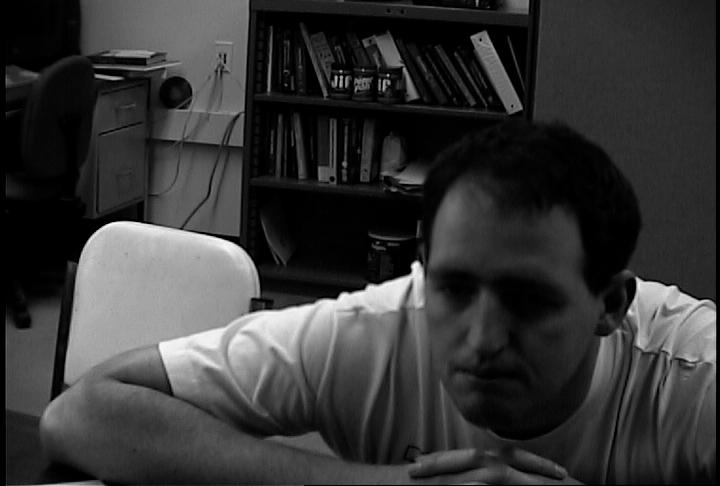
\includegraphics [width=4in]{rightDan.jpg}
\end{center}
\caption{Original Image.  This image is the original image. }
\label{rightDan}
\end{figure}

\begin{figure}[htb]
\begin{center}
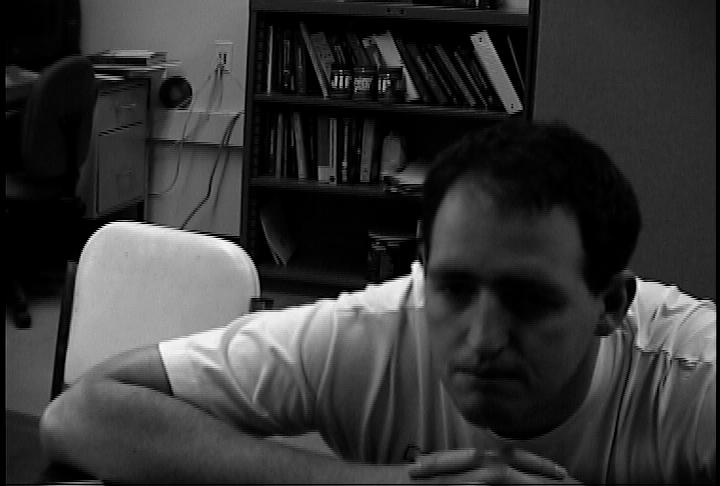
\includegraphics [width=4in]{revRecover.jpg}
\end{center}
\caption{Recovered Image.  This image is the recovered image.  Depending on whether the image was saved as a picture first can affect the white spots in the picture.  Ringing is also an issue.  }
\label{rightDanRecovered}
\end{figure}

\begin{figure}[htb]
\begin{center}
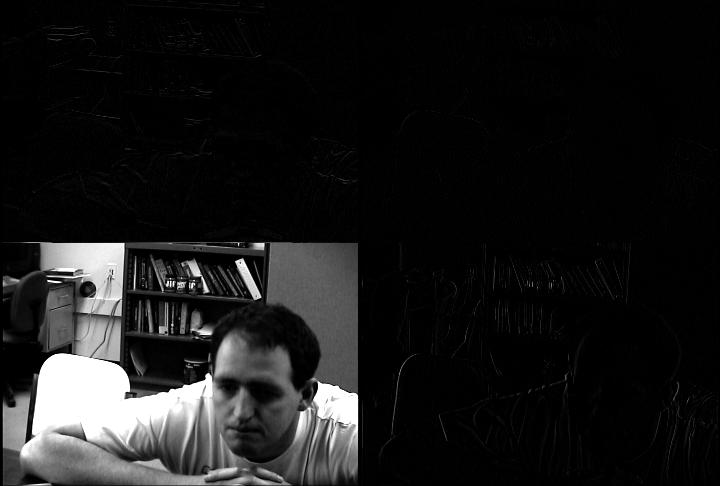
\includegraphics [width=4in]{revWavepic.jpg}
\end{center}
\caption{Wavelet Transform Image.  This image is divided in to average, horizontal, vertical and diagonal components. }
\label{rightWavepic}
\end{figure}

%Note: April 11, 2003:  Proofed up to this point

\begin{figure}[htb]
\begin{center}
\includegraphics [width=4in]{selfWavepic.jpg}
\end{center}
\caption{Wavelet Transform Image.  This image is divided in to average, horizontal, vertical and diagonal components, using the vector-matrix version. }
\label{wavepic}
\end{figure}

\begin{figure}[htb]
\begin{center}
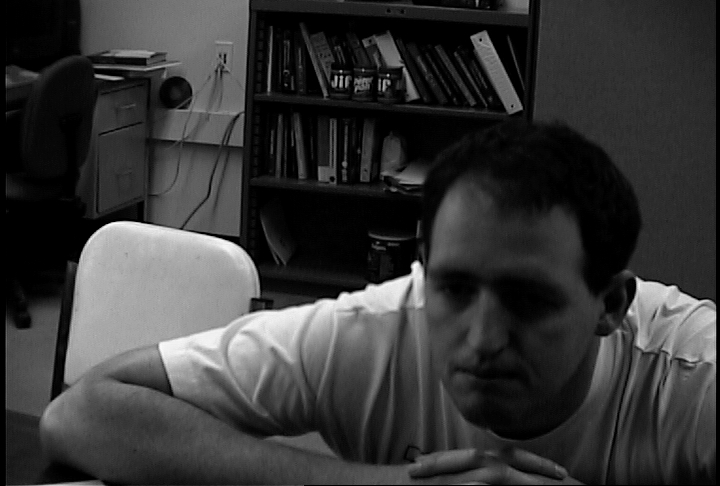
\includegraphics [width=4in]{selfRecover.jpg}
\end{center}
\caption{Recovered Image (Vector-Matrix Method).  This image is the recovered image.  This version avoids the ringing by using the vector-matrix version which is more aligned for the inverse wavelet transform.  }
\label{selfRecover}
\end{figure}


\subsection {Multiresolution Results}
The expected result is a picture within a picture.  Each average component has a further transform on it.  The three resolution transform has the form:
\[
\left(\begin{array}{cccccccc}A_3 & V_3 & V_2 &  & V_1 &  &  &  \\H_3 & D_3 &  &  &  &  &  &  \\H_2 &  & D_2 &  &  &  &  &  \\ &  &  &  &  &  &  &  \\H_1 &  &  &  & D_1 &  &  &  \\ &  &  &  &  &  &  &  \end{array}\right)
\]
%\[
%W_3 = 
%\left(
%\begin{array}{cc}
%\left(
%\begin{array}{cc}
%\left(
%\begin{array}{cc}
%A_3& V_3 \\ 
%H_3 & D_3
%\end{array} 
%\right)
%V_2 \\ 
%H_2 & D_2
%\end{array}
%\right)
% & V_1 \\ 
%H_1 & D_1
%\end{array}
%\right)
%\]
Refer to Figure \ref{wavepicR3} for the image transform results.  

\begin{figure}[htb]
\begin{center}
\includegraphics [width=4in]{wavepic3R.jpg}
\end{center}
\caption{Wavelet Transform Image.  This image is divided in to average, horizontal, vertical and diagonal components using multiresolution wavelet transform.  Note the the average component was transformed one step further. }
\label{wavepicR3}
\end{figure}

\begin{figure}[htb]
\begin{center}
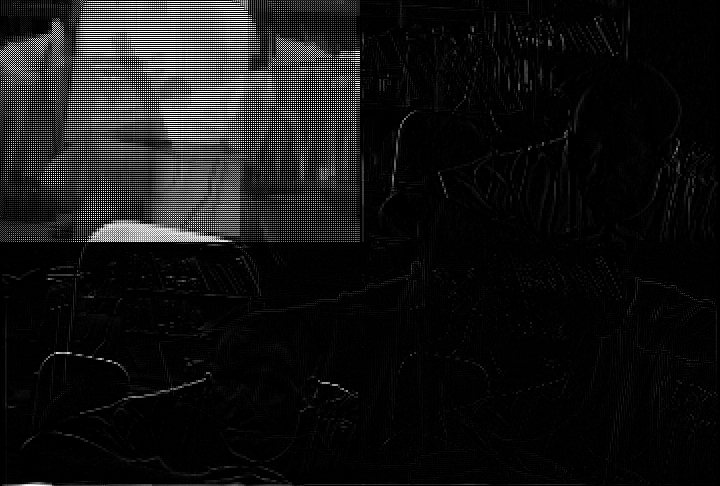
\includegraphics [width=4in]{recoverHid.jpg}
\end{center}
\caption{Recovered Image - Wrong Order (Multiresolution). This image shows a 2D wavelet transform after it was recovered out of order.  Obviously, the distortion is hideous.  }
\label{recoverHid}
\end{figure}

To obtain the inverse, an exact reverse procedure is necessary, otherwise the distortion is hideous.   The first attempt of the wavelet inverse transform was out of order, refer to Figure \ref{recoverHid}.  A correct picture was obtained during the second attempt.  Correct order yielded correct results, refer to Figure \ref{rightDanRecovered}.



\subsection {Threshold Filtering}
After a triple resolution, a 0.02 threshold will eliminate 81.1706 percent of elements in the original sample picture.  Also at this point, the effects of removing these elements becomes visually evident (Figure \ref{recover3R002}).  At a 0.01 threshold,  66.0205 percent of the elements are removed.  Visually, the recovered sample and the original appear to be the same (Figure \ref{recover3R001}).  At a threshold of 0.1, 92.9987 percent of the elements are reduced to zero.  However, the distortions are clearly visible at this level of thresholding (Figure \ref{recover3R010}).  Even at a threshold of 0.001 which is below the numerical precision of the original, 16.0814 elements are reduced to zero.  At a threshold of 0.002, 28.9683 percent is removed.  

Consequently after a triple resolution, nearly 29\% of the data was irrelevant for the image's brightness resolution (which also applies to color).  Subjective examination reveals that removing 60\% to 85\% of the data was not noticeable to human perception.  Which leaves only 15\% to 40\% of the data actually contributing or being necessary to reconstruct the image.   

\begin{figure}[htb]
\begin{center}
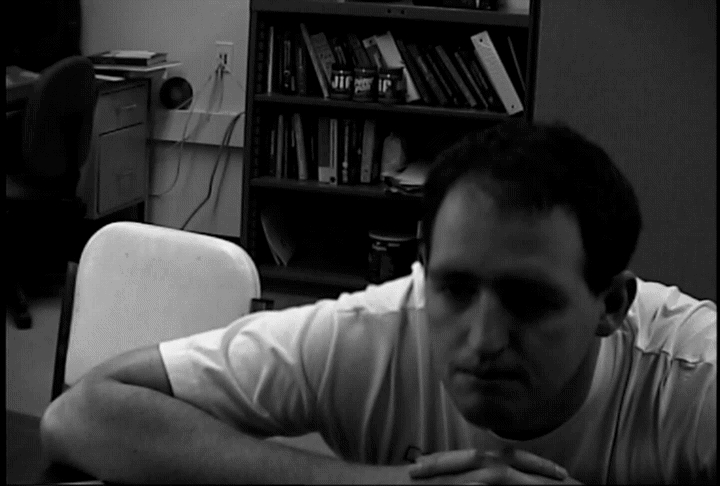
\includegraphics [width=4in]{recover3R002T.jpg}
\end{center}
\caption{Recovered Image - 2\% threshold (Multiresolution). This image had nearly 83\% of its elements removed in the triple resolution wavelet transform.  }
\label{recover3R002}
\end{figure}


\begin{figure}[htb]
\begin{center}
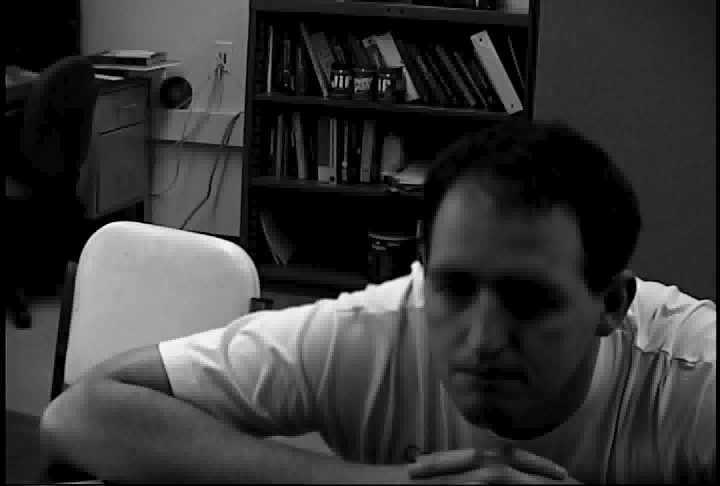
\includegraphics [width=4in]{recover3R010T.jpg}
\end{center}
\caption{Recovered Image - 10\% threshold (Multiresolution). This image had nearly 93\% of its elements removed in the triple resolution wavelet transform.  }
\label{recover3R010}
\end{figure}


\begin{figure}[htb]
\begin{center}
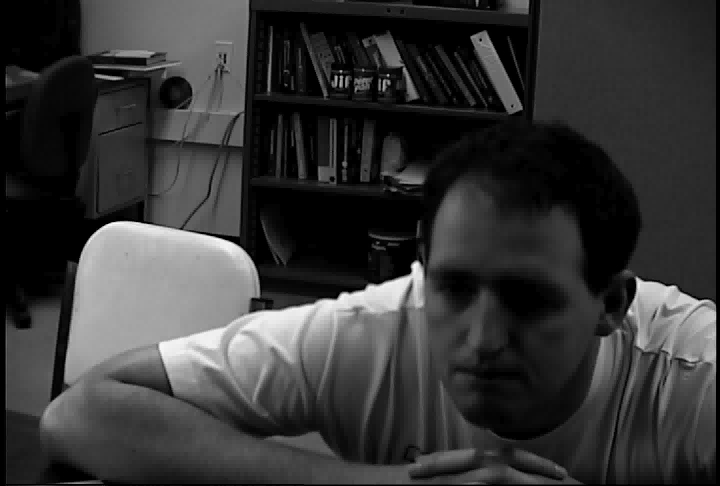
\includegraphics [width=4in]{recover3R005T.jpg}
\end{center}
\caption{Recovered Image - 5\% threshold (Multiresolution). This image had nearly 85\% of its elements removed in the triple resolution wavelet transform.    }
\label{recover3R005}
\end{figure}


\begin{figure}[htb]
\begin{center}
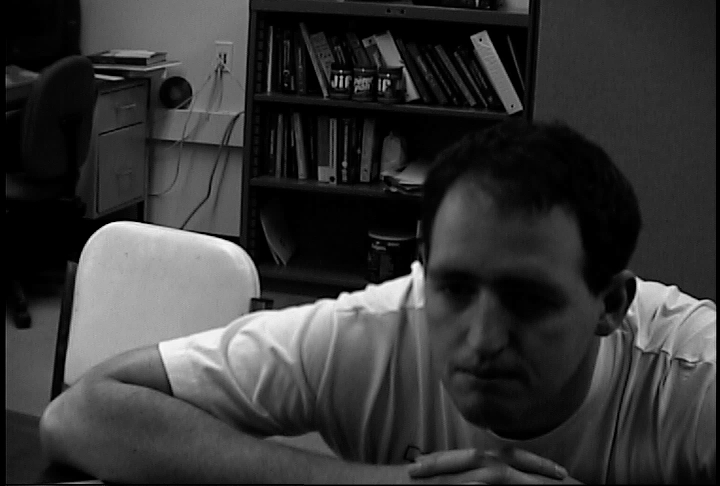
\includegraphics [width=4in]{recover3R001.jpg}
\end{center}
\caption{Recovered Image - 1\% threshold (Multiresolution).  This image had nearly 60\% of its elements removed in the triple resolution wavelet transform.   }
\label{recover3R001}
\end{figure}



\chapter {Matrix Multiplication via Wavelets}
%\documentclass[11pt]{article}
%\usepackage{graphicx}
%\usepackage{amssymb}
%\usepackage{epstopdf}
%\DeclareGraphicsRule{.tif}{png}{.png}{`convert #1 `dirname #1`/`basename #1 .tif`.png}

%\textwidth = 6.5 in
%\textheight = 9 in
%\oddsidemargin = 0.0 in
%\evensidemargin = 0.0 in
%\topmargin = 0.0 in
%\headheight = 0.0 in
%\headsep = 0.0 in
%\parskip = 0.2in
%\parindent = 0.0in

%\newtheorem{theorem}{Theorem}
%\newtheorem{corollary}[theorem]{Corollary}
%\newtheorem{definition}{Definition}

%\title{Brief Article}
%\author{The Author}
%\begin{document}
%\maketitle

In this chapter, the general concept of matrix multiplication via
wavelets is introduced. First, matrix multiplication and sparse matrix
multiplication itself is reviewed for completeness.  Then the $\psi^n$
transform with the Haar basis is shown to provide a precodnitioned
matrix which can be used to compute the matrix product. The correctness
of this method is demonstrated through a formal proof.

\section{Matrix Multiplication}

Matrix multiplication is one of the fundamental operations in linear algebra.  It is defined for two matrices $A$ and $B$, denoted $C = A\cdot B$.  Matrix multiply requires that the row length of A to be the same as the column length of B.  The value of element, $c_{i,j}$ is defined by
\[
c_{i,j} = \sum\limits_k a_{i,k} b_{k,j}.
\]
Matrix multiplication also obeys the following properties \cite{lipschutz}.
\begin{itemize}
\item Associative law:  $(AB)C = A(BC)$
\item Left Distributive Law $A (B+C) = AB + AC$
\item Right Distributive Law $(B+C)A = BA + CA$
\item Distribution of a constant
\end{itemize} 
For two generic $2 \times 2$ matrices, $A$ and $B$, the resulting products is
\begin{equation}\displaystyle
\label{eqn:conventional}
A \cdot B = 
\left(\begin{array}{cc}  a^1_1&  a^2_1 \\ a^1_2 &  a^2_2 \end{array}\right)
\left(\begin{array}{cc}  b^1_1&  b^2_1 \\ b^1_2 &  b^2_2 \end{array}\right) =
\left(\begin{array}{cc}  a^1_{1} b^1_{1} + a^2_{1} b^1_{2}&  a^1_{1}b^2_{1} + a^2_{1}  b^2_{2}    \\ a^1_{2} b^1_{1} + a^2_{2} b^1_{2} &  a^1_{2} b^2_{1} + a^2_{2} b^2_{2} 
\end{array}\right).
\end{equation}


There is a fast matrix multiplication which was devised in 1969 by  Strassen.  It achieves a computational complexity of $O(N^{2.807})$ for large $N$ representing one dimension of the matrix.  This works for square matrices.  There is a variation of the Strassen called the Winograd which obtains slightly better performance  \cite{lederman}.

Another view on matrix multiplication is sparse multiplication. The
whole point of sparse matrix multiplication is to take a matrix such
that the matrix composition is mostly zero, and exploit that
composition to reduce the number of multiplications required.  Such
multiplication schemes optimal limit for matrix multiplication is
$O(N^2)$. One method is included in the Sparse Matrix Multiplication
Package, called SYMBMM \cite {bank}. Another is contained in the Basic
Linear Algebra Subprogram for sparse matrix to dense matrix multiply.


%\bibitem {blackford} Z. Bai, J. Demmel, J. Dongarra, A. Ruhe, and H. van der Vorst, editors. \textsl {Templates for the Solution of Algebraic Eigenvalue Problems: a Practical Guide}. SIAM, Philadelphia, 2000.

%\bibitem {bank} Randolph E. Bank, Craig C. Douglas \textsl{Sparse Matrix Multiplication Package} April 23, 2001.

%\bibitem {lederman} Steven Huss-Lederman, Elaine M. Jacobson, J.R. Johnson, Anna Tsao, Thomas Turnbull \textsl {Strassen's Algorithm for Matrix Multiplication: Modeling, Analysis, and Implementation} November 15, 1996


\section {Wavelet Matrix Multiplication}
The point of this thesis is not show the efficiencies of these above algorithms.  Rather, it is to show a pre-conditioner using the wavelet transform that can be used in each of them.  %In the process examples of multi-resolution schemes that do not work shall be exposed.  The ones that work will be examined for fidelity and accuracy as elements are cast away.
Wavelet based matrix multiply is sound for the Haar Wavelet Transform and the $\psi^n$ expansion.   
%Wavelet based matrix multiplication is sound only as long as the wavelet operator is a linear operator.   Any optimizer applying the wavelet transform must ensure linearity is maintained.  
If the Haar Wavelet Transform produces a sparse and well conditioned matrix, then the Haar Wavelet Transform proves itself as a useful preconditioner.  %sparseness and a well conditioned matrix result in the process, then the resulting matrix should be simpler to multiply.    
Here, the general concept of matrix multiplication via wavelets is introduced, and the linearity principle is shown.  
%One of t
The key point for wavelet matrix multiplication is the proof that $W(A) \times W(B) = W(A\times B)$  If this is the case, then it is obvious that $W(A) \times W(B) = W(\Gamma) = W(A\times B = \Gamma)$.  %So far the proof is still weak.  The reason is that an example proof is useful for proving something to not be the case, rather than being the case.   However, a simple example does show some intuitive steps that would be necessary for a proof.  



\subsection{A $2\times 2$ example}

The feasibility of multiplication in the wavelet domain is demonstrated directly using a $2 \times 2$ matrix. The coefficients of the matrices are multiplied both according to normal matrix multiplication and the modified wavelet multiplication operator. In the end the resulting coefficients are seen to be the same.

\subsubsection{Wavelet Transforms of the Matrices}

For a wavelet transform, the result on matrix $A$ is
\begin{equation} \label{WA} \displaystyle
W(A) = 
{1 \over 2} 
\left(\begin{array}{cc}  
\left(a^1_1 + a^1_2 + a^2_1 + a^2_2\right) & 
\left(a^1_1 + a^1_2 - a^2_1 - a^2_2\right)  \\ 
\left(a^1_1 - a^1_2 + a^2_1 - a^2_2\right) & 
\left(a^1_1 - a^1_2 - a^2_1 + a^2_2\right)   
\end{array}\right), 
\end{equation}
and for matrix $B$ it is
\begin{equation} \label{WB} \displaystyle
W(B) = {1 \over 2} 
\left(\begin{array}{cc}
\left(b^1_1 + b^1_2 + b^2_1 + b^2_2\right) &
\left(b^1_1 + b^1_2 - b^2_1 - b^2_2\right) \\ 
\left(b^1_1 - b^1_2 + b^2_1 - b^2_2\right) &  
\left(b^1_1 - b^1_2 - b^2_1 + b^2_2\right)
\end{array}\right).
\end{equation}

\subsubsection{Product of $A$ and $B$ in wavelet space}

The conventional product of $A$ and $B$ (equation \ref{eqn:conventional}) can be transformed into wavelet space. The wavelet transform of this matrix is represented by 
\[
W(A \cdot B) =
{1 \over 2}
\left(
\begin{array}{cc}
\psi(A) & \psi(V) \\
\psi(H) & \psi(D)
\end{array}
\right)
\]
where 
\begin{eqnarray}
\label{eqn:abwavelet1}
\psi(A) &=& (a^1_1 b^1_1 + a^2_1 b^1_2 + a^1_1b^2_1 + a^2_1  b^2_2) + (a^1_2 b^1_1 + a^2_2 b^1_2 + a^1_2 b^2_1 + a^2_2 b^2_2)\\
\label{eqn:abwavelet2}
\psi(V) &=&(a^1_1 b^1_1 + a^2_1 b^1_2  - a^1_1b^2_1 - a^2_1  b^2_2) +  (a^1_2 b^1_1 + a^2_2 b^1_2 - a^1_2 b^2_1 - a^2_2 b^2_2 ) \\
\label{eqn:abwavelet3}
\psi(H) &=& (a^1_1 b^1_1 + a^2_1 b^1_2 + a^1_1b^2_1 + a^2_1  b^2_2) - (a^1_2 b^1_1 + a^2_2 b^1_2 + a^1_2 b^2_1 + a^2_2 b^2_2)\\
\label{eqn:abwavelet4}
\psi(D) &=& (a^1_1 b^1_1 + a^2_1 b^1_2  - a^1_1b^2_1 - a^2_1  b^2_2) - (a^1_2 b^1_1 + a^2_2 b^1_2 - a^1_2 b^2_1 - a^2_2 b^2_2 ).
\end{eqnarray}

\subsubsection{The product of the waveletized matrices}

Straight forward multiplication of $W(A) \cdot W(B)$ represented by equations \ref{WA} and \ref{WB} works out as follows:
\[
W(A) \cdot W(B) = 
{1 \over 4} 
\left(
\begin{array}{cc}
W_A & W_V \\
W_H & W_D
\end{array}
\right)
\]
where
\begin{eqnarray*}
W_A &=& (a^1_1 + a^1_2 + a^2_1 + a^2_2)( b^1_1 + b^1_2 + b^2_1 + b^2_2) + ( a^1_1 + a^1_2 - a^2_1 - a^2_2)(b^1_1 - b^1_2 + b^2_1 - b^2_2) \\
W_V &=& ( a^1_1 + a^1_2 + a^2_1 + a^2_2) ( b^1_1 + b^1_2 - b^2_1 - b^2_2) + (a^1_1 + a^1_2 - a^2_1 - a^2_2) ( b^1_1 - b^1_2 - b^2_1 + b^2_2)  \\
W_H &=&  ( a^1_1 - a^1_2 + a^2_1 - a^2_2)(b^1_1 + b^1_2 + b^2_1 + b^2_2) +  ( a^1_1 - a^1_2 - a^2_1 + a^2_2 ) (b^1_1 - b^1_2 + b^2_1 - b^2_2) \\
W_D &=& ( a^1_1 - a^1_2 + a^2_1 - a^2_2) (b^1_1 + b^1_2 - b^2_1 - b^2_2)+( a^1_1 - a^1_2 - a^2_1 + a^2_2 )(b^1_1 - b^1_2 - b^2_1 + b^2_2)
\end{eqnarray*}
which simplifies to
\begin{eqnarray*}
W_A &=& a^1_1 b^1_1 + a^1_2 b^1_1 + a^2_1 b^1_2 + a^2_2 b^1_2 + a^1_1 b^2_1 + a^1_2 b^2_1 + a^2_1 b^2_2 + a^2_2 b^2_2 \\
W_V &=& a^1_1 b^1_1 + a^1_2 b^1_1 + a^2_1 b^1_2 + a^2_2 b^1_2 - a^1_1 b^2_1 - a^1_2 b^2_1 - a^2_1 b^2_2 - a^2_2 b^2_2 \\
W_H &=& a^1_1 b^1_1 - a^1_2 b^1_1 + a^2_1 b^1_2 - a^2_2 b^1_2 + a^1_1 b^2_1 - a^1_2 b^2_1 + a^2_1 b^2_2 - a^2_2 b^2_2 \\
W_D &=& a^1_1 b^1_1 - a^1_2 b^1_1 + a^2_1 b^1_2 - a^2_2 b^1_2 - a^1_1 b^2_1 + a^1_2 b^2_1 - a^2_1 b^2_2 + a^2_2 b^2_2 
\end{eqnarray*}
These can then be compared to the coefficients of $W(A \cdot B)$ in equations \ref{eqn:abwavelet1}-\ref{eqn:abwavelet2} and seen to be identical. This asserts that $W(A) \cdot W(B) = W(A \cdot B)$ in the case of $2 \times 2$ matrices.

\subsection{Haar Wavelet Multiplication}

Given that the multiplication of the transformed coefficients is the
same as the transformation of the multiplied coefficients, an
algorithm can be developed to take advantage of this. The Haar Wavelet
Multiplication Algorithm is presented in Algorithm
\ref{alg:haarwaveletmultiply}. This produces a correct solution. 

\begin{algorithm}
\caption{ Haar Wavelet Multiplication}
\label{alg:haarwaveletmultiply}
\begin{algorithmic}
\REQUIRE Matrices $A$ and $B$
\STATE $\hat A \leftarrow \psi^n(A)$
\STATE $\hat B \leftarrow \psi^n(B)$
\STATE $\hat C \leftarrow \hat A \cdot \hat B$
\STATE $C \leftarrow \psi^{-n}\left(\hat C\right)$
\end{algorithmic}
\end{algorithm}

However, the preconditioned matrix has not been sparsified. In order to
sparsify the matrix, it is thresholded. Then, only nonzero elements are
retained and sparse matrix matrix multiplication can be employed on the
previously dense matrix. This is presented in Algorithm \ref{alg:sparsehaarmultiply}.


\begin{algorithm}
\caption{ Sparse Haar Wavelet Multiplication}
\label{alg:sparsehaarmultiply}
\begin{algorithmic}
\REQUIRE Matrices $A$ and $B$
\STATE $\hat A \leftarrow \psi^n(A)$
\STATE $\hat B \leftarrow \psi^n(B)$
\STATE $l_A \leftarrow$ sparsify $\left(\hat A\right)$
\STATE $l_B \leftarrow$ sparsify $\left(\hat B\right)$
\STATE $l_C \leftarrow$ sparse multiply $\left(l_A, l_B \right)$
\STATE $\hat C \leftarrow$ densify $\left(\hat C \right)$
\STATE $C \leftarrow \psi^{-n}\left(\hat C\right)$
\end{algorithmic}
\end{algorithm}
	

\section{Formal Proof of the Haar Wavelet Multiplication}

The formal proof of the correctness of the haar wavelet multiplication is presented below.


\subsection {Haar Wavelets and Vector Inner Products}
One of the other crucial keys for the Haar Wavelet Transform Matrix Multiply to work is vector inner product.  The issue is whether or not 
\begin{equation}
\langle f', g' \rangle = \langle f,g \rangle 
\end{equation}
is true for vectors $f$ and $g$ which both of length $p$, and the wavelet transformed versions of $f$ and $g$ denoted $f'$ and $g'$ respectively.
To show this, $\langle f',g' \rangle$ is expanded algebraically to establish its identity.  
\begin{equation}
\label {vectinwt}
\langle f',g' \rangle = \sum \limits_{k=0} ^{p/2 -1}(\frac{f_{2k} +f_{2k+1}}{\sqrt{2}} \cdot \frac{g_{2k} + g_{2k+1}}{\sqrt{2}}) + \sum \limits_{k=0} ^{p/2 -1}(\frac{f_{2k} - f_{2k+1}}{\sqrt{2}} \cdot \frac{g_{2k} - g_{2k+1}}{\sqrt{2}})
\end{equation}
When equation \ref{vectinwt} is expanded further, the terms that emerge expose the identity of the inner product.  
\begin{eqnarray}
\label {vectinwte}
\langle f',g' \rangle = \frac{1}{2}  \sum \limits_{k=0} ^{p/2 -1}
( f_{2k} g_{2k} + f_{2k+1}g_{2k} + f_{2k}g_{2k+1} + f_{2k+1}g_{2k+1}  \\ \nonumber+  f_{2k} g_{2k} - f_{2k+1}g_{2k} - f_{2k}g_{2k+1} + f_{2k+1}g_{2k+1} 
\end{eqnarray}
When simplified the $f_{2k}g_{2k+1}$ and $f_{2k+1}g_{2k}$ terms cancel.  The $f_{2k}g_{2k}$ and $f_{2k+1}g_{2k+1}$ terms combine to yield equation \ref{vectinwtsimple} and further simplifies to equation {vectinwtsimple2}.
\begin{equation}
\label {vectinwtsimple}
\langle f',g' \rangle = \frac{1}{2}  \sum \limits_{k=0} ^{p/2 -1} (f_{2k}g_{2k} + f_{2k+1}g_{2k+1})
\end{equation}
\begin{equation}
\label {vectinwtsimple2}
\langle f',g' \rangle = \frac{1}{2}  \sum \limits_{k=0} ^{p-1} (f_{k}g_{k} ) = \langle f,g \rangle
\end{equation}


\subsection{Matrix Multiply with the Haar Transform: Formal Proof}
\textbf{Given} two arbitary matrices $A$ of size $m\times p$, $B$ of size $m\times p$, the Haar Wavelet Pair, and the Haar Wavelet Transform.  The wavelet pair to be used here is 
\[ \psi_H (x)= \sqrt{\frac{1}{2}} \left\{\begin{array}{cc}1 & x=0 \\-1 & x=1 \\0 & otherwise\end{array}\right.\]
\[\phi_H (x) = \sqrt{\frac{1}{2}} \left\{\begin{array}{cc}1 & x=0 \\0 & otherwise\end{array}\right. \]  
%Vectors: f, g
%N $\times$ N matrices: A, B
%

Also, this notation is used for this proof.
\begin{itemize}
\item $\psi_{1R}(S)$ is the row transform of matrix $S$.
\item $\psi_{1C}(S)$ is the column transform of matrix $S$.
\item $\psi {S}$ is the 2-D wavelet transform of matrix $S$.
\item $\langle f,g \rangle = \langle \psi_1(f) , \psi_1(g) \rangle $
\item $A' = \psi(A)$
\item $B' = \psi(B)$
\item $A^R =\psi_{1R}(A) $
\item $B^C =\psi_{1C}(B) $ 
\item $A^R_{ri}$ is the row vector $i$ of the row transform of $A$.
\item $A^R_{ri+1}$ is the row vector $i+1$ of the row transform of $A$.
\item $B^C_{cj}$ is the column vector $j$ of the column transform of $B$
\item $B^C_{cj+1}$ is the column vector $j+1$ of the column transform of $B$
\end{itemize}

\textbf{Required} show that 
\[ \psi (A) \psi (B) = \psi (A B) \]
is a true statement. %One fact that may also be useful is: \[ \left\leftangle \psi_1(f), \psi_1(g) \right\rightangle \ \equiv \left\leftangle f, g \right\rightangle \]


\textbf{Proof}

There are two formulae required for transforming either A or B into the wavelet domain.
\begin{equation}
\label{wavedefc4A}
 \psi (A) = \psi _{1R} ( \psi_{1C} (A)) = \psi _{1C} ( \psi_{1R} (A))
\end{equation}
\begin{equation}
\label{wavedefc4B}
\psi (B) = \psi _{1R} ( \psi_{1C} (B)) = \psi _{1C} ( \psi_{1R} (B))    
\end{equation}

Thus, this is simply a re-write of the definition of the wavelet transform by the CWT.   Next,  define a matrix $\Gamma'$  so that
\[\Gamma' = \psi (A) \psi (B) \].  From, the definition $\Gamma'$, a series of re-writes and the properties of the Haar Wavelet Transform can expose the solution for every element of $\Gamma'$ and $\Gamma'$.  In general, the elements of $\Gamma'$ defined as follows:
\begin{equation}
\label{wavecrossA}
\Gamma'_{i,j} =   \left\langle \psi_{1C} (\psi_{1R} (A)) _{ri} , \psi_{1R} (\psi_{1C} (B)) _{ci}  \right\rangle
\end{equation}
\begin{equation}
\label{wavecrossB}
\Gamma'_{i,j} =   \left\langle \psi_{1R} (\psi_{1C} (A)) _{ri} , \psi_{1C} (\psi_{1R} (B)) _{ci}  \right\rangle
\end{equation}

In this case, each element of $\Gamma'$ is defined as nothing more than the inner product of row $i$ of $\psi(A)$ and column $j$ of $\psi(B)$.  This is in agreement with standard matrix multiplication.  %In this case, discrete (vector) inner product is the inner product form being used, and is defined for vectors $f$ and $g$ of length $n$
%\begin{equation}
%\label{innerproduct}
%\langle f, g\rangle =  \sum_{k=1} ^n f_k \cdot g_k
%\end{equation}
%
%Another re-write of $\Gamma'$ now is in order.  This re-write uses the definition of inner product  along with results of the Haar Transform.

%\[  \left\langle A'_{ri} , B'_{cj}  \right\rangle =  \sum\limits_{k=0}^{row/2-1}\frac{1}{2}%
%((A^R_{ri})_{k}+(A^R_{ri})_{k+1})((B^C_{cj})_{k}+(B^C_{cj})_{k+1}))  + \sum\limits_{k=0}^{row/2-1}\frac{1}{2}%
%((A^R_{ri})_{k}-(A^R_{ri})_{k+1})((B^C_{cj})_{k}-(B^C_{cj})_{k+1})) \]
%The re-write of $\Gamma'$ reduces the operation to a one-dimensional wavelet transform.  Now four cases are established by the follow definitions for the Haar Wavelet Transform (in one-dimension) for either column transforms or row transforms:
Another identity that is important what the wavelet pair for transform will do in either a row or column transform.  
\[  \psi _{1C} (A) = \left\{ 
\begin{array}{ll}
\frac{A_{i,j}+A_{i,j+1}}{\sqrt{2}} & j<col \\ 
\frac{A_{i,j}-A_{i,j+1}}{\sqrt{2}} & j\geq col%
\end{array}
\right.   \]
 \[  \psi _{1R} (A) = \left\{ 
\begin{array}{ll}
\frac{A_{i,j}+A_{i+1,j}}{\sqrt{2}} & i<row \\ 
\frac{A_{i,j}-A_{i+1,j}}{\sqrt{2}} & i\geq row%
\end{array}
\right. 
 \]
 %insert table for cases
 
In this case, there are four cases to show for:
\begin{enumerate}
\item $i < \frac{row}{2}$ and $j <  \frac{col}{2}$
\item $i \geq \frac{row}{2}$ and $j <  \frac{col}{2}$
\item $i < \frac{row}{2}$ and $j \geq  \frac{col}{2}$
\item $i \geq \frac{row}{2}$ and $j \geq  \frac{col}{2}$
\end{enumerate}

 \textbf{Case 1} $i < \frac{row}{2} $ and $j < \frac{col}{2}$.
The base equation $\Gamma'_{i,j}$ in this cases is as follows:
\begin{equation}
\label{case1inner}
 \Gamma'_{ij} = \left\langle \frac {A^R_{ri} + A^R_{ri+1}}{\sqrt{2}} , \frac {B^C_{cj} + B^C_{cj + 1}}{\sqrt{2}} \right\rangle
\end{equation}

%This definition is valid of $i\in [0,\frac{r_l}{2} -1]$ and $j\in [0, 
This re-write must be expanded to expose an equality.  This expansion is valid for vectors sums within inner products.   Thus $\Gamma'_{i,j}$ in this case is expanded to:
\[ \Gamma'_{i,j} = \frac{1}{2} ( \left\langle A^R_{ri}, B^C_{cj}   \right\rangle +   \left\langle A^R_{ri+1}, B^C_{cj}   \right\rangle +  \left\langle A^R_{ri}, B^C_{cj + 1}   \right\rangle +  \left\langle A^R_{ri+1}, B^C_{cj+1}   \right\rangle    ) \]

Next, $\Gamma'_{i,j}$ must be compared to $\psi(\Gamma)_{i,j}$ where
\[ \psi (A B)  = \psi (\Gamma)    \]
By definition, every element in $C$ is defined:
\[ C_{i,j} =   \left\langle A_{ri} , B_{cj}  \right\rangle \]
The next step is to show what every element within this case is for $\psi(\Gamma)$.  This is done by analyzing what the column transform will do at $C_{i,j}$.  To do this, the column transform is applied to both column $j$ and $j+1$ for columns between $[0,\frac{col}{2} -1]$.  The effects of these column transforms are defined in equations \ref{rowwtC1c1} and \ref{rowwtC2c1}.
\begin{equation}\displaystyle
\label {rowwtC1c1}
 \psi_{1C} (\Gamma)_{i,j} = \frac{1}{\sqrt{2}} \left\langle A_{ri} , B_{cj}  \right\rangle + \left\langle A_{ri +1} , B_{cj}  \right\rangle 
\end{equation}
\begin{equation}
\label {rowwtC2c1}
\psi_{1C} (\Gamma)_{i,j+1} = \frac{1}{\sqrt{2}} \left\langle A_{ri} , B_{cj+1}  \right\rangle + \left\langle A_{ri +1} , B_{cj+1}  \right\rangle \
\end{equation}

The result of the row transform on $\psi_{1C}(\Gamma)$ in this case is a sum of $\psi_{1C}(\Gamma)_{i,j}$ and $\psi_{1C}(\Gamma)_{i,j+1}$, and specified in equation \ref{rowtfCc1}.
\begin{equation}
\label{rowtfCc1}
 \psi(\Gamma) = \frac{1}{\sqrt {2}} (\psi_{1C} (\Gamma)_{i,j} + \psi_{1C} (\Gamma)_{i,j+1}   )
\end{equation}
 Expanded this equation is equation \ref{rowtfCc1e}.
\begin{equation}
\label{rowtfCc1e}
 \psi(\Gamma) = \frac{1}{2} (  \left\langle A_{ri} , B_{cj}  \right\rangle + \left\langle A_{ri +1} , B_{cj}  \right\rangle + \left\langle A_{ri} , B_{cj+1}  \right\rangle + \left\langle A_{ri +1} , B_{cj+1}  \right\rangle   ) 
\end{equation}


\textbf{Case 2} $i \geq \frac{row}{2}$ and $j <  \frac{col}{2}$.
The base equation $\Gamma'_{i,j}$ in this cases is as follows:
\[ \Gamma'_{ij} = \left\langle \frac {A^R_{ri,j} - A^R_{ri+1}}{\sqrt{2}} , \frac {B^C_{cj} + B^C_{cj + 1}}{\sqrt{2}} \right\rangle  \]
The next step is to show what every element within this case is for $\psi(\Gamma)$.  
\[ \Gamma'_{i,j} = \frac{1}{2} ( \left\langle A^R_{ri}, B^C_{cj}   \right\rangle -   \left\langle A^R_{ri+1}, B^C_{cj}   \right\rangle +  \left\langle A^R_{ri}, B^C_{cj + 1}   \right\rangle -  \left\langle A^R_{ri+1}, B^C_{cj+1}   \right\rangle    ) \]
How does this compare with $\psi (\Gamma)$?
\[ \psi (A B)  = \psi (\Gamma)    \]
\[ (\Gamma) = \psi  \left\langle A_{ri} , B_{cj}  \right\rangle \]
This equation expands with wavelet operator to:
\[ \psi_{1C} (\Gamma)_{i,j} = \frac{1}{\sqrt{2}} \left\langle A_{ri} , B_{cj}  \right\rangle - \left\langle A_{ri +1} , B_{cj}  \right\rangle   \]
\[ \psi_{1C} (\Gamma)_{i,j+1} = \frac{1}{\sqrt{2}} \left\langle A_{ri} , B_{cj+1}  \right\rangle - \left\langle A_{ri +1} , B_{cj+1}  \right\rangle \  \]

The result of the row transform on $\psi_{1C}(\Gamma)$ in this case is a sum of $\psi_{1C}(\Gamma)_{i,j}$ and 
\[ \psi(\Gamma) = \frac{1}{\sqrt {2}} (\psi_{1C} (\Gamma)_{i,j} + \psi_{1C} (\Gamma)_{i,j+1}   ) \]

 Expanded this equation is equation \ref{rowtfCc1e}.
\[ \psi(\Gamma) = \frac{1}{2} (  \left\langle A_{ri} , B_{cj}  \right\rangle - \left\langle A_{ri +1} , B_{cj}  \right\rangle + \left\langle A_{ri} , B_{cj+1}  \right\rangle - \left\langle A_{ri +1} , B_{cj+1}  \right\rangle   ) \]

\textbf {Case 3} $i < \frac {row}{2}$ and $j \ge \frac{col}{2}$.
Like, before the base case for $\Gamma'_{i,j}$
\[ \Gamma'_{ij} = \left\langle \frac {A^R_{ri,j} + A^R_{ri+1}}{\sqrt{2}} , \frac {B^C_{cj} - B^C_{cj + 1}}{\sqrt{2}} \right\rangle  \]
Again, the vector sums are expanded within their inner products.  
\[ \Gamma'_{i,j} = \frac{1}{2} ( \left\langle A^R_{ri}, B^C_{cj}   \right\rangle +   \left\langle A^R_{ri+1}, B^C_{cj}   \right\rangle -  \left\langle A^R_{ri}, B^C_{cj + 1}   \right\rangle -  \left\langle A^R_{ri+1}, B^C_{cj+1}   \right\rangle    ) \]
Next, $\Gamma'_{i,j}$ is compared with $\psi(\Gamma)$
\[ \psi (A B)  = \psi (\Gamma)    \]
Next, the column transform expansion is conducted:
\[ (\Gamma) = \psi  \left\langle A_{ri} , B_{cj}  \right\rangle \]
\[ \psi_{1C} (\Gamma)_{i,j} = \frac{1}{\sqrt{2}} \left\langle A_{ri} , B_{cj}  \right\rangle + \left\langle A_{ri +1} , B_{cj}  \right\rangle   \]
\[ \psi_{1C} (\Gamma)_{i,j+1} = \frac{1}{\sqrt{2}} \left\langle A_{ri} , B_{cj+1}  \right\rangle + \left\langle A_{ri +1} , B_{cj+1}  \right\rangle \  \]
Now the column transform results are combined, by subtraction in this case:
\[ \psi(\Gamma) = \frac{1}{\sqrt {2}} (\psi_{1C} (\Gamma)_{i,j} - \psi_{1C} (\Gamma)_{i,j+1}   ) \]
Lastly, the expanded form is expanded.
\[ \psi(\Gamma) = \frac{1}{2} (  \left\langle A_{ri} , B_{cj}  \right\rangle + \left\langle A_{ri +1} , B_{cj}  \right\rangle - \left\langle A_{ri} , B_{cj+1}  \right\rangle - \left\langle A_{ri +1} , B_{cj+1}  \right\rangle   ) \]

 \textbf{Case 4} $i \ge \frac {row}{2}$ and $j \ge \frac{col}{2}$.
Like, before the base case for $\Gamma'_{i,j}$ 
\[ \Gamma'_{ij} = \left\langle \frac {A^R_{ri,j} - A^R_{ri+1}}{\sqrt{2}} , \frac {B^C_{cj} - B^C_{cj + 1}}{\sqrt{2}} \right\rangle  \]
Again, the vector sums are expanded within their inner products. 
\[ \Gamma'_{i,j} = \frac{1}{2} ( \left\langle A^R_{ri}, B^C_{cj}   \right\rangle -   \left\langle A^R_{ri+1}, B^C_{cj}   \right\rangle -  \left\langle A^R_{ri}, B^C_{cj + 1}   \right\rangle +  \left\langle A^R_{ri+1}, B^C_{cj+1}   \right\rangle    ) \]

Next, $\Gamma'_{i,j}$ is compared with $\psi(\Gamma)$
\[ \psi (A B)  = \psi (\Gamma)    \]
\[ (\Gamma) = \psi  \left\langle A_{ri} , B_{cj}  \right\rangle \]
Once the column wavelet transform expands $\Gamma$ to
\[ \psi_{1C} (\Gamma)_{i,j} = \frac{1}{\sqrt{2}} \left\langle A_{ri} , B_{cj}  \right\rangle - \left\langle A_{ri +1} , B_{cj}  \right\rangle   \]
\[ \psi_{1C} (\Gamma)_{i,j+1} = \frac{1}{\sqrt{2}} \left\langle A_{ri} , B_{cj+1}  \right\rangle - \left\langle A_{ri +1} , B_{cj+1}  \right\rangle \  \]

Now the column transform results are combined, by subtraction in this case:
\[ \psi(\Gamma) = \frac{1}{\sqrt {2}} (\psi_{1C} (\Gamma)_{i,j} - \psi_{1C} (\Gamma)_{i,j+1}   ) \]

Lastly, the expanded form is expanded.
\[ \psi(\Gamma) = \frac{1}{2} (  \left\langle A_{ri} , B_{cj}  \right\rangle - \left\langle A_{ri +1} , B_{cj}  \right\rangle - \left\langle A_{ri} , B_{cj+1}  \right\rangle + \left\langle A_{ri +1} , B_{cj+1}  \right\rangle   ) \]

Since the inner product of two vectors $f,g$ is the same as their wavelet transformed vectors $f',g'$, then all 4 cases produce a case where $\Gamma'_{i,j} = (\psi (\Gamma))_{i,j} \ \forall (i,j)$.  Thus for the Haar Wavelet Transform (discrete mother basis), 
\[ \psi (A) \cdot \psi(B) = \psi (A\cdot B) \].

\section {Multi Resolution Expansion Proof}
In a previous section, wavelet based matrix multiplication was proven such that
\[\psi(A) \cdot \psi(B) = \psi (A\cdot B) \]
In this section the question of whether or not there is MRE form which is sound for matrix multiplication.  There are few facts that are relevant and were made obvious in the empirical analysis in the results %section of this 
chapter.  
\begin{itemize}
\item $\psi_{WPx} (A) \not= \psi^x(A) $  where $\psi_{WPx} (A) $ is the $x$ resolution of wavelet transform packets (full decomposition) except for $x=1$.
\item $\psi_{Wx} (A) \not= \psi^x(A) $  where $\psi_{Wx} (A) $ is the $x$ resolution of wavelet transform pyramids except for $x=1$.
\end{itemize}

The next hypothesis to be answered is can the wavelet transform be applied more than once to condition a matrix for matrix multiplication?  This question is answered by the following lemma.

\[ \psi ^2 (A) \cdot \psi^2 (B)  = \psi^2(A\cdot B) \]
Proof: \\
%\begin{enumerate}
%\item 
%\end{enumerate}
The theorem \[ \psi(A) \cdot \psi(B) = \psi (A\cdot B) \] is proven as fact.
\[ \psi^2(A) = \psi(\psi (A))\]
\[ \psi^2 (A) =\cdot \psi^2 (B) = \psi(\psi(A)) \cdot \psi (\psi (B))  \]
\[ \psi(\psi(A)) \cdot \psi (\psi (B)) = \psi (\psi(A) \cdot \psi(B) ) \]
\[ \psi (\psi(A) \cdot \psi(B) ) = \psi (\psi(A \cdot (B))  \]
\[ \psi (\psi(A \cdot (B)) = \psi^2(A \cdot B) \]
Therefore: 
\[ \psi ^2 (A) \cdot \psi^2 (B)= \psi^2(A \cdot B) \]


 

% \end{document}


\chapter {Results} \label{chp:results}
%\documentclass[11pt]{article}
%\usepackage{graphicx}
%\usepackage{amssymb}
%\usepackage{epstopdf}
%\usepackage{doublespace}
%\DeclareGraphicsRule{.tif}{png}{.png}{`convert #1 `dirname #1`/`basename #1 .tif`.png}

%\textwidth = 6.5 in
%\textheight = 9 in
%\oddsidemargin = 0.0 in
%\evensidemargin = 0.0 in
%\topmargin = 0.0 in
%\headheight = 0.0 in
%\headsep = 0.0 in
%\parskip = 0.2in
%\parindent = 0.0in

%\newtheorem{theorem}{Theorem}
%\newtheorem{corollary}[theorem]{Corollary}
%\newtheorem{definition}{Definition}

%\title{Matrix Multiply Results}
%\author{Daniel D. Beatty}
%\begin{document}
%\maketitle

%\chapter


Each empirical result is from % either 
a series of matrix multiplications on 9 different images.  These matrices were submitted preconditioning with the wavelet transform in the 3 basic method of decomposition, wavelet pyramid, wavelet packet (full decomposition) and the $\psi^n$ decomposition.%   with wavelet packets or wavelet pyramids type wavelet transforms.  
In the end, wavelet pyramids performed poorly for any set of resolutions deeper than one in matrix multiplication.  Thus wavelet packets should not be used as a pre-conditioner to matrix multiplication.  The wavelet transform  by wavelet packets performs modestly in matrix multiplication tests, but to be effective must be reordered into $\psi^n$ structure. %require reordering to match the recursive MRE wavelet transform packet form.    
Lastly, the $psi^n$ form performs well on matrix multiply.   

The matrix multiply used in each of these cases is %a special case of matrix multiply is conducted, 
$A^2= A\cdot A$, where $A$ is $M\times N$ The general equation for evaluating the wavelet transform pyramid method is the fidelity measurement:

\[\sqrt{E(\psi_{Pr}^{-x} ( (\psi_{Pr}^x (A))^2) - A^2)} \]

Relative Fidelity measurements provide a relative standard and is more useful for general observations.  To obtain this measurement, the results are compared to standard.% reference of a standard.  
In this case, $A^2$ is the standard, and the energy difference is relative to that standard.  

\[ \sqrt {\frac{E(\psi_{Pr}^{-x} ( (\psi_{Pr}^x (A))^2) - A^2)} {E(A^2)} }  \]

%\section {Matrix Multiplication Results}
%\{tiny}

\section {Empirical Analysis: Wavelet Transform Pyramids}

Several standard images were used for measuring effect matrix multiply in each of these multiplications.  Amongst them were the artificial images such as the waterfall and the clock.  Others were actual images such as an arial view of the Pentagon, an in flight photo of an F-16, a fishing boat, an opera house, a river, and a set of bell peppers.

In first round analysis, matrix multiply was measured against the wavelet pyramids.  These showed some undesirable results.  As the decomposition proceeded deeper, the fidelity quick became unstable, and made the method unusable for matrix multiplication.  

These tables are shown below.

Sample Two: Peppers $512 \times 512$ by wavelet transform pyramid 

\begin{tabular}{llll}
{Resolution} & { Original Energy } & { 
Estimate Energy }& { 
Fidelity } \\ 
1&  12972.4& 12972.4 &  $1.26464 \cdot 10^{-13} $ \\ 
2&12972.4  & 12960.3 &  3.11211  \\ 
3& 12972.4 &12947.8  &  5.44678  \\ 
4&12972.4&12939.7&   8.43738 \\
5 &12972.4  & 12926 & 13.1662 \\
6& 12972.4& 12904.3& 19.9257 \\
7& 12972.4 & 12877.9 & 25.4429 \\
\end{tabular}


%Sample Three: Molly Holly $256 \times 256$ by wavelet transform pyramid 

%\begin{tabular}{lllll}
%{\tiny Number of Resolution} & {\tiny Original Energy }$E(O)$ & {\tiny 
%Estimate Energy }$E(\widetilde{O})$ & $(E(O)-E(\widetilde{O}))$ & {\tiny 
%Fidelity }$\sqrt{E((O)-(\widetilde{O}))}$ \\ 
%$1$ & $582.864 $ & $582.864$ &  $-9.75244\cdot 10^{-16}$ & $2.0396 \cdot 10^{-14}$ \\ 
%$2$ & $582.864 $& $583.05 $  & $-0.000319839$ & $1.19806 $  \\ 
%$3$ &  $582.864$ & $582.613$ & $0.000430391$  & $2.18712$ \\ 
%$4$ & $582.864$ & $579.473$ & $0.00581664$ &  $3.19317$ \\ 
%$5$ & $582.864$ & $576.72$ & $0.0105413$ & $4.82652$ 

%\end{tabular}


Sample Four: Waterfall $512 \times 512$ by wavelet transform pyramid 

\begin{tabular}{llll}
{ Resolution} & { Original Energy }& { 
Estimate Energy } &  { 
Fidelity } \\ 
$1$&  $6630.76$ & $6630.76$&  $9.37836e-14$ \\ 
$2$& $6630.76$ & $6629.92$  &  $1.20049$ \\ 
$3$& $6630.76$ & $6626.6$   & $2.37529$ \\ 
$4$& $6630.76$ & $6619.14$  & $3.9194$ \\ 
$5$& $6630.76$ & $6595.14$  &  $6.63615$\\ 
$6$& $6630.76$ & $6579.62$  & $9.48774$ \\ 
$7$& $6630.76$ & $6567.17$  &  $12.1211$
\end{tabular}

\section {Empirical Analysis: Wavelet Transform Packets}
The primary example shown is from the Peppers image.  Although, all nine of the images used for this thesis could have been used, all of them exhibit similar qualities.   After, two resolutions the 2-D MRE becomes unstable for matrix multiplication.  It misplaces sections to where random noise in those sections would be just useful as the actual information contained in those sections.  
%These examples were chosen arbitrarily from a selection images with fidelity-issued features.  In other-words, a loss in fidelity is noticed by the human eye.  Also, size was considered in these measurements as well.  

Sample One: Peppers $512 \times 512$ by wavelet transform packet 

\begin{tabular}{llll}
{ Resolution } &  {Original Energy }  &{ Estimate Energy }  & {Fidelity} \\ 
$1$ & $12972.4$ &  $12972.4$ &  $1.26464e \cdot 10^{-13}$\\ 
$2$ & $12972.4$ & $12972.4$ &  $0.059622$ \\ 
$3$ & $12972.4$ & $12972.4$ &  $0.072957$  \\ 
$4$& $12972.4$  & $12972.4$  & $0.0849579$  \\ 

$5$& $12972.4$  & $12972.4$  & 0.09721  \\ 

$6$& $12972.4$  & $12972.4$ &  $0.104528$  \\ 

$7$& $12972.4$  & $12972.4$ &  $0.119789$  \\ 

\end{tabular}

\section {Empirical Results on the Psi-N Wavelet Transform Method}
The Psi-N transform clearly produces better results as shown in all examples of the wavelet transform.  Trade off issues start to appear when comparing the number of resolution levels to apply as opposed to a spare filter threshold.   

In these next examples, resolution levels 1 through 7 are examined by removing data based on energy level.  The method used is to strictly remove the lower threshold of energy from the matrix at large.  %The second method removes energy first by eliminating whole segments.  The third is a hybrid, removing first the segments at large and then filtering on the threshold segment.  
The range of energy thresholds vary from 0 to $\frac{9}{10}$. 

The reasoning for any of these schemes is to establish sparse representations of the matrix.  In these sparse representation, only the above threshold elements are used.   These representations are useful for sparse matrix multiplication since only the above threshold elements need be multiplied thus reducing the number of multiplications (operations at large) performed.  

%\subsubsection {Strict Lower Threshold Scheme: The Darwin Filter}
This filter is appropriately named for allowing the strongest elements to survive and weaker ones to be reduced to zero.  This particular Darwin Filter is applied through out the matrix.  In order to find the element that is the threshold element, each element in the matrix is squared, placed in a one dimensional array, and then sorted in the array from least to greatest.  %Lastly the summing loop is applied to the array, and is stopped when either entire array is processed or the sum has reached the threshold value.  The threshold value is established by the energy of the matrix multiplied by the energy percentage to be removed.  
Lastly, two method exist to find the threshold value in the array of values.  One is to sum up values until the threshold energy level has been reached.  Another is to take element relative to the percentage threshold desired.  The relative percentage method is simpler, by performing one division on the energy array size and a look up for the value in the energy array.  

Once found, the filter threshold is used to filter out elements whose squared value is less than the threshold.  Those elements that are less are made to be zero.   Those that are above the threshold are left alone.  

For this experiment both matrix operands have the filter applied.  It should be noted that for the BLAS level three matrix multiply, this filtering scheme need only be applied to the first matrix operand.   Applying this filter to the second is simply unnecessary since the method states that the second matrix can be dense.  

The pattern of fidelity loss has a dramatic climb in the first $\frac{1}{20}$ of energy loss.  From $\frac{1}{20}$ th to $\frac{1}{2}$ the fidelity stays roughly within the same order of magnitude.  After this there is a sharp rise until all fidelity is lost.  

\begin{figure}
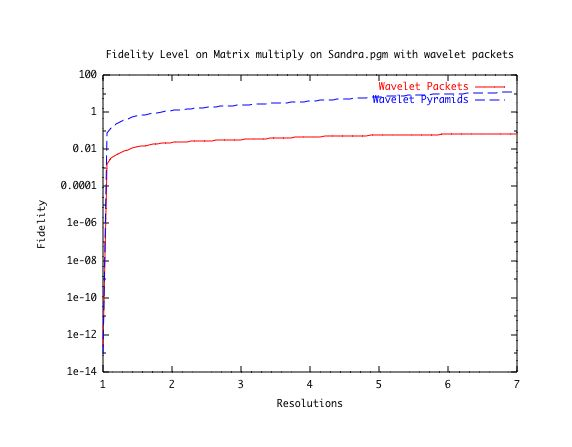
\includegraphics [width=7in]{sandrapyrpackresults.jpg}
\caption{This fidelity level graph shows that the wavelet transform packet method as a preconditioner to matrix multiply is not reliable past the first resolution. The wavelet packet produces marginal results mostly due sections being placed out of order.}
\label{packetresultsstraight}
\end{figure}






\begin{figure}
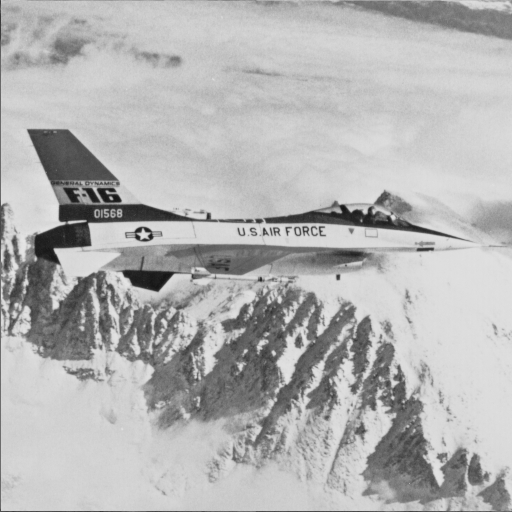
\includegraphics [width=3in]{f16.jpg}
\caption{This image is a photo of an F-16 fighter jet provided Courtesy of the Signal and Image Processing Institute at the University of Southern California.  \cite{f16}}
\label{image f16}
\end{figure}


\begin{figure}
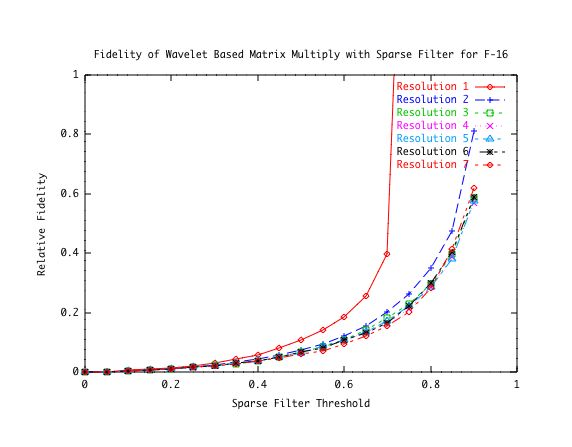
\includegraphics [width=5.5in]{f16resultsA.jpg}
\caption{This fidelity level graph shows that Psi Wavelet Transform (full decomposition) approximation error in matrix multiplication.  This graph in particular was obtained by multiplying the F-16 image by itself with various resolution levels of Wavelet Transforms applied. \cite{f16} }
\label{image f16 fidelity}

\end{figure}

\begin{figure}
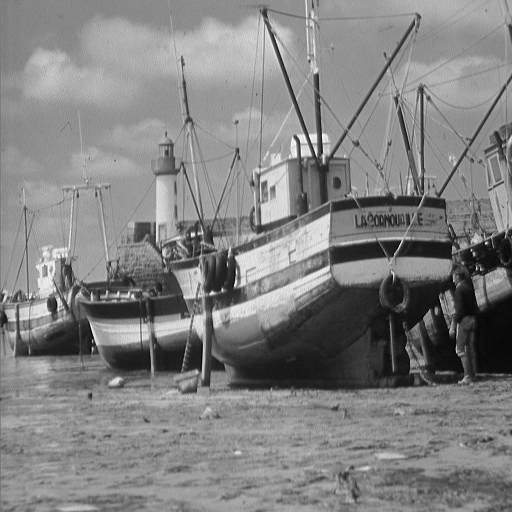
\includegraphics [width=3in]{fishingboat.jpg}
\caption{This image is a photo of an F-16 fighter jet provided Courtesy of the Signal and Image Processing Institute at the University of Southern California.  \cite{fishingboat}}
\label{image_fishingboat}
\end{figure}



\begin{figure}
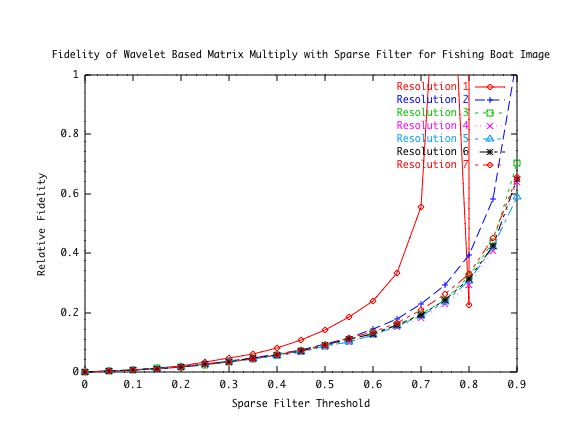
\includegraphics [width=5.5in]{fishingboatresultA.jpg}
\caption{This fidelity level graph shows that Psi Wavelet Transform (full decomposition) approximation error in matrix multiplication.  This graph in particular was obtained by multiplying the Fishing Boat image by itself with various resolution levels of Wavelet Transforms applied. \cite{fishingboat}  }
\label{image_fishingboat_fidelity}
\end{figure}


\begin{figure}
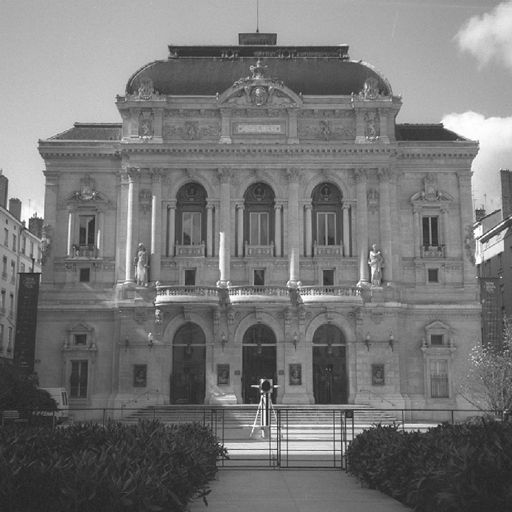
\includegraphics [width=3in] {opera.jpg}
\caption {This image is a photo of the Opera House in Lyon \cite{opera}}
\label{Opera House}
\end{figure}

\begin{figure}
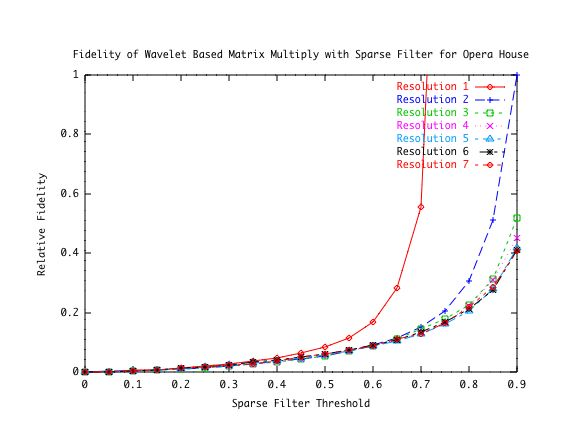
\includegraphics [width=5.5in]{operaresultsA.jpg}
\caption{This fidelity level graph shows that Psi Wavelet Transform (full decomposition) approximation error in matrix multiplication.  This graph in particular was obtained by multiplying the Opera House image by itself with various resolution levels of Wavelet Transforms applied.  }
\label{image_opera_fidelity}
\end{figure}

\begin{figure}
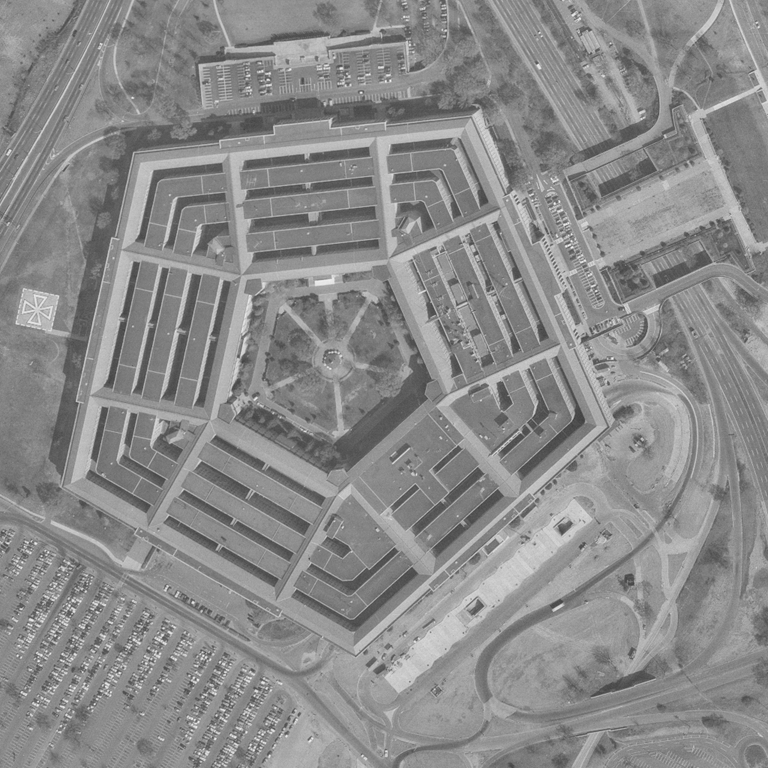
\includegraphics [width=3in]{pentagon.jpg}
\caption{This image is an ariel photo of an Pentagon provided Courtesy of the Signal and Image Processing Institute at the University of Southern California.  \cite{pentagon}}
\label{image fishingboat}
\end{figure}

\begin{figure}
\includegraphics [width=5.5in]{pentagonresultsA.jpg}
\caption{This fidelity level graph shows that Psi Wavelet Transform (full decomposition) approximation error in matrix multiplication.  This graph in particular was obtained by multiplying the Pentagon image by itself with various resolution levels of Wavelet Transforms applied. \cite{Pentagon} }
\label{image_pentagon_fidelity}
\end{figure}

\begin{figure}
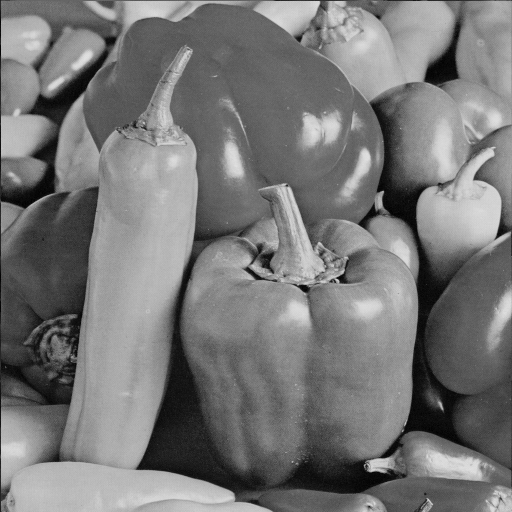
\includegraphics [width=3in]{peppers.jpg}
\caption{This image is an ariel photo of  ``Peppers'' provided Courtesy of the Signal and Image Processing Institute at the University of Southern California.  \cite{peppers}}
\label{image Peppers}
\end{figure}

\begin{figure}
\includegraphics [width=5.5in]{peppersresultsA.jpg}
\caption{This fidelity level graph shows that Psi Wavelet Transform (full decomposition) approximation error in matrix multiplication.  This graph in particular was obtained by multiplying the Peppers image by itself with various resolution levels of Wavelet Transforms applied. \cite{peppers} }
\label{image_peppers_fidelity}
\end{figure}

\begin{figure}
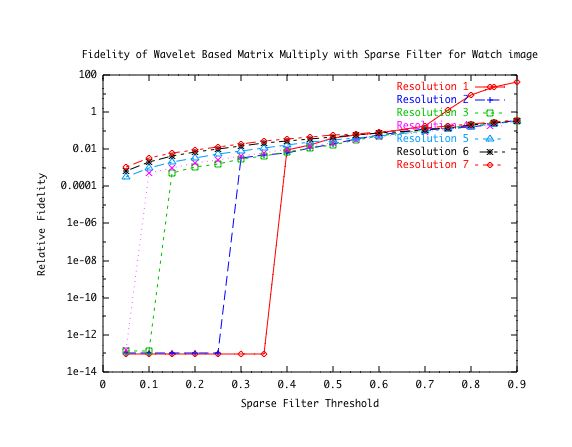
\includegraphics [width=6in]{watchResultsA.jpg}
\caption{This fidelity level graph shows that Psi Wavelet Transform (full decomposition) approximation error in matrix multiplication.  This graph in particular was obtained by multiplying the Watch image by itself with various resolution levels of Wavelet Transforms applied.  \cite{watch} }
\label{image_watch_fidelity}
\end{figure}

\begin{figure}
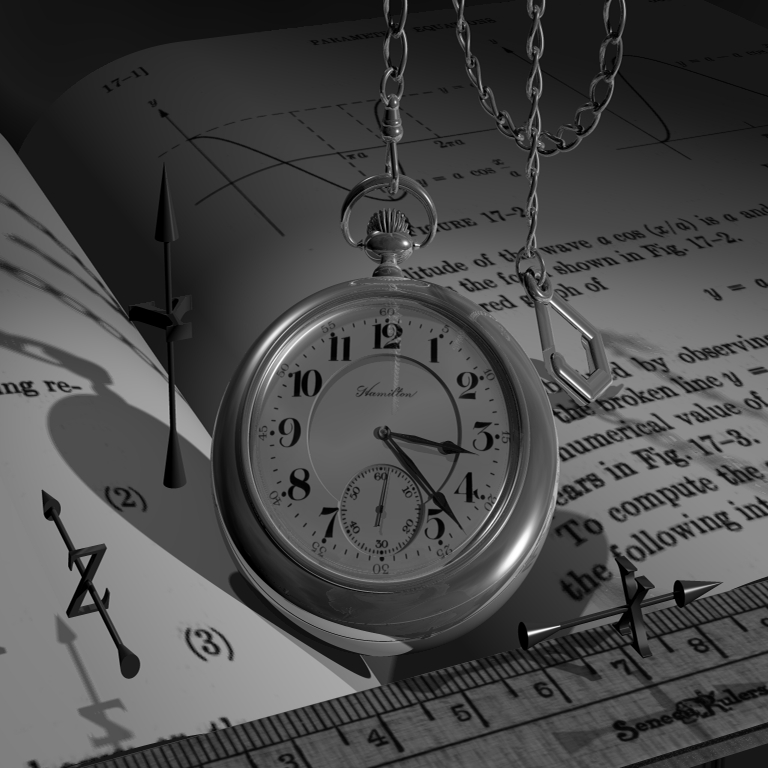
\includegraphics [width=3in]{watch.jpg}
\caption{``Pocket Watch on a Gold Chain. Copyright image courtesy of Kevin Odhner''   \cite{watch}}
\label{image Peppers}
\end{figure}

\begin{figure}
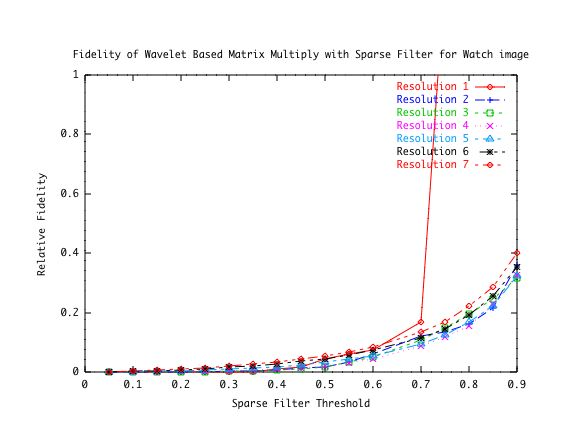
\includegraphics [width=4in]{watchResultsB.jpg}
\caption{This fidelity level graph shows that Psi Wavelet Transform (full decomposition) approximation error in matrix multiplication.  This graph in particular was obtained by multiplying the Watch image by itself with various resolution levels of Wavelet Transforms applied.  \cite{watch}  }
\label{image_watch_fidelity}
\end{figure}

\begin{figure}
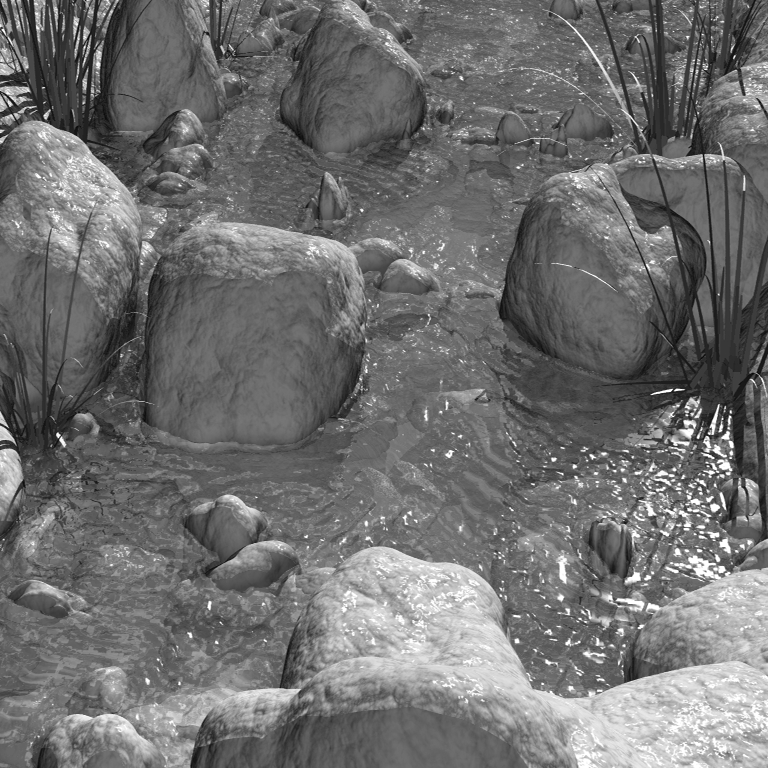
\includegraphics [width=3in]{water.jpg}
\caption{This image is an ariel photo of  ``Always running, never the same....'' provided Courtesy of the Jaime Vives Piqueres.  \cite{water}}
\label{image Peppers}
\end{figure}

\begin{figure}
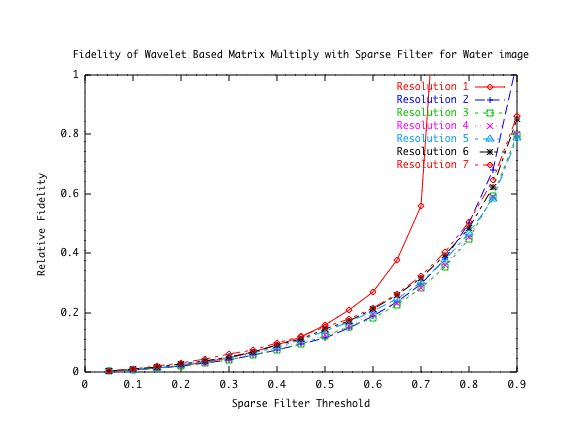
\includegraphics [width=6in]{waterResultsA.jpg}

\caption{This fidelity level graph shows that Psi Wavelet Transform (full decomposition) approximation error in matrix multiplication.  This graph in particular was obtained by multiplying the Water image by itself with various resolution levels of Wavelet Transforms applied.  \cite{watch} }
\label{image_waterfall_fidelity}
\end{figure}


\begin{figure}
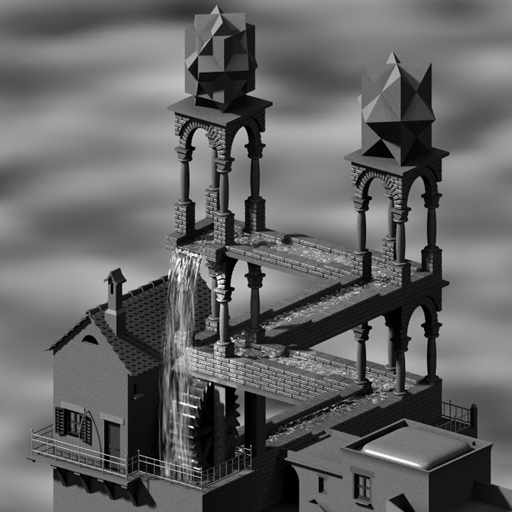
\includegraphics [width=3in]{waterfall.jpg}
\caption{"This is a raytraced version of M.C.Escher's (1898-1972) famous lithography
'Waterfall' (1961), which again is based on a spatial illusion drawen by the
mathematician Roger Penrose." \cite{waterfall} }
\label{image waterfall}
\end{figure}
\begin{figure}
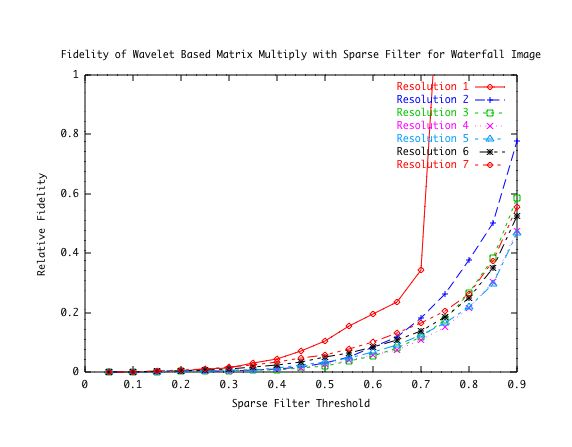
\includegraphics [width=3in]{waterfallResultsA.jpg}
\caption{This fidelity level graph shows that Psi Wavelet Transform (full decomposition) approximation error in matrix multiplication.  This graph in particular was obtained by multiplying the Waterfall image by itself with various resolution levels of Wavelet Transforms applied.  \cite{waterfall} }
\label{image_waterfall_fidelity}
\end{figure}

%\begin{thebibliography}{99}
%\bibitem {waterfall} Sascha Ledinsky \textsl{Waterfall} http://oz.irtc.org/ftp/pub/stills/1998-10-31/waterfa1.txt Internet Raytracing Competition copyright October 31, 1998
%\bibitem {water} Jaime Vives Piqueres \textsl {Always running, never the same...} http://oz.irtc.org/ftp/pub/stills/1998-10-31/running.txt  Internet Raytracing Competition copyright October 31, 1998
%\bibitem {watch} Kevin Odhner \textsl {Pocket Watch on a Gold Chain} 
%\bibitem {opera} fabien a. p. petitcolas {Opera House of Lyon} open domain
%\bibitem {pentagon} Signal and Image Processing Institute at the University of Southern California \textsl{Pentagon} The copyright status of this images in unclear.
%\bibitem {f16}  Signal and Image Processing Institute at the University of Southern California \textsl{F-16}
% The copyright status of this images in unclear.
%\bibitem  {peppers} Signal and Image Processing Institute at the University of Southern California \textsl {Peppers} The copyright status of this images in unclear.
%\bibitem {fishingboat} Signal and Image Processing Institute at the University of Southern California \textsl {Fishing Boat} The copyright status of this images in unclear.

%\end {thebibliography}
% \end{document} 

\chapter {Conclusion}
These following items shall be accomplished by this thesis:  testing matrix multiplication and testing partial differential equations with the wavelet transform as a preconditioning function.  The hypothesis for matrix multiplication is that a sparser matrix should emerge and therefore should be easier to multiply.  In case of the partial differential equation, the hypothesis is that  a better conditioned matrix should emerge.
%\begin{enumerate}
%\item Matrix Multiplication
%\item Wavelet Based Partial Differential Equation
%\end{enumerate}

In order to satisfy the matrix multiplication component, a prototype shall be developed.  This prototype shall multiply two matrices together.  Several wavelet bases shall be used to condition the matrix.  The results shall be tested for their correctness.  

For the wavelet based partial differential equation, another prototype shall be developed.  This prototype shall solve the PDE within the standard implicit method to provide means of comparison.  A few wavelet basis function shall be used to test their effectiveness in solving PDE.  Also, a few multi-resolution methods shall be used to test their effectiveness.  


%\backmatter

%\appendix
%\chapter{Wavelets Implemented in General}
\section{Haar Wavelet Transform Class:}

\bigskip The Haar Wavelet Transform class has the purpose of taking in a
signal and outputing the signal processed by the Haar Wavelet Transform. \
It is dependent on the convolution function for computation. \ It is also
dependent on the haar function generator to establish a Haar Scaling and
Wavelet vector. \ For practical I/O, a result plotter is also necessary. \ 

\bigskip All of the above can be accommodated within one class. \ One other
class that is necessary is the myVector class. \ This class provides a
simple, yet practical data type for the computation. \ It can be allocated
and deallocated such that its size is appropriate for the task. \ 

It is projected that the two-dimensional version will simply add a matrix
manipulator. \ What such a manipulator extracts rows and columns into
myVector structures such that the computation to procede on each row and
column.. \ 

\subsection{\protect\bigskip One Dimensional Wavelet Transform}

The primary function in the Wavelet transform class is the one dimensional
wavelet transform (hWaveXform). \ More than one form of this function could
possible exist; however, for simplisty only one was produced. \ It takes two
myVector classes (input and output). \ It produces a haar difference and
scaling vector, as well as a $R_{A}$, $R_{D}$, $T$, $F$ and $S$ myVector
classes for use within the function. \ The algorithm is as follows

$S=input$

$l=$ is the size of S (or the input)

$\forall i\in \lbrack 0,l)$

\qquad $R_{A}=S\ast H_{A}$

\qquad $R_{D}=S\ast H_{D}$

\qquad T = join ($R_{A}$,$R_{D}$)

\qquad F = evenSplit (T)

\qquad ForceInsert (F, output)

\qquad end = floor ( $\frac{l}{2^{i+1}}$)

\qquad Extract (output, S, 0, end)

\bigskip

The Extract procedure is to take values from output up to the index end, and
make S a copy of that vector. \ Thus S is called the resolution vector. \ T
is always twice the size of the working S vector. \ F is always half. \ The
resolution vector decreases by half each iteration, and starts at the same
size as the input.

\bigskip

\subsection{Join Procedure}

The join procedure is rather simple. \ Produce a result whose size is the
size of the two sources combined, and whose elements are those of the two
input vectors. \ 

Input:

\qquad myVector left, right

Output:

\qquad myVector Result

Algorithm

\qquad result.deallocate

\qquad $s_{l\,}=size(left)$

\qquad $s_{r}=size(right)$

\qquad $s=s_{l}+s_{r}$

\qquad result.allocate(s)

\qquad $\forall i\in \lbrack 0,s_{l})$

\qquad \qquad result[i]=left[i]

\qquad $\forall i\in \lbrack s_{l},s)$

\qquad \qquad result[i]= right$[i-s_{l}]$

\subsection{Procedure: Even Split}

This procedure is simply a special type for condensing procedure. \ Simply
put, this procedure makes the result half the size of the original input. \
Both the input and result are myVector classes. \ The characteristic of the
elements of the result is:

\qquad result[i] = input[2*i]

\subsubsection{Input:}

\qquad myVector s

\subsubsection{Output:}

\qquad myVector r

\subsubsection{Algorithm}

\qquad l = ceil (s.size/2)

\qquad r.allocate(l)

\qquad $\forall i\in \lbrack 0,l)$

\qquad \qquad $r_{i}=s_{i\ast 2}$

\bigskip

\bigskip

\subsection{Procedure: Force Insert}

\bigskip Purpose: To insert one myVector ,s, into a larger myVector, r. \
The constraint is that r be larger than s. \ As long as this is the case,
then forced insertion can occur. \ Special cases can include start and end
points. \ In which case, the start and end points must be within the
specified range.

\subsubsection{Input:}

\qquad myVector s, r

\subsubsection{Output:}

\qquad myVector r

\subsubsection{Algorithm:}

\qquad $l_{1}=s.size$

\qquad $l_{2}=r.size$

\qquad if ($l_{1}<l_{2}$) and (start < end)

\qquad \qquad $\forall i\in \lbrack start,end]$

\qquad \qquad \qquad $r_{i}=s_{i}$

\bigskip

\subsection{Procedure: Extract}

Purpose: To produce a new or replace a myVector whose length is that of the
section to copied and extracted. \ The point behind this procedure is
provide allow a wavelet transform to be performed on a segment of data, and
keep the procedure the same each resolution. \ 

\bigskip

\subsubsection{Input:}

The inputs for the wavelet Xform extraction procedure are as
follows:

\qquad myVector S,

\qquad integer a \ 

\qquad integer b \ 

These names are arbitray. \ The variables a and b specify the start and end
points respectively. \ Obviously, there is an inequality relationship here.

\qquad $0\leq a\leq b\leq S.size$

\bigskip

\subsubsection{Output:}

The output of the wavelet Xform > extraction procedure is
simply:

\qquad myVector R

The elements of R are a copy of the elements of S from index a to index b.

\bigskip

\subsubsection{Algorithm}

\qquad if ( 0 <a < b < S.size)

\qquad \qquad R.deallocate

\qquad \qquad l = b - a +1

\qquad \qquad R.allocate(l)

\qquad \qquad $\forall i\in \lbrack a,b]$

\qquad \qquad \qquad $R_{i-a}=S_{i}$

\bigskip


\subsection {Procedure: Haar Wavelet Inverse (Left Side)}
Purpose:  These procedures are specific case toward the 2-element Haar Wavelet.  They take in an array of even length and return an array of equal size which is the Inverse Haar Wavelet Transform of the original.  The format of the original is assumed to be ($A|D_{1}|D_{2}|...|D_{n}$).

\subsubsection {Input}
A "MyVector" class which is an array with simple operations associated with it.   The object name is source.  The source is of the form ($A|D_{1}|D_{2}|...|D_{n}$).  

\subsubsection{Output} 
A "MyVector"  class with an object name of result.  

\subsubsection{Algorithm}
There is a difference between the current algorithm and the ideal algorithm which may be the source of error.  This algorithm uses the following symbols to aide in its description:
\begin{itemize}
\item S is the source myVector
\item A is the average term for which $A_i = S_i$ \newline
\item D is the difference term for which $D_i = S_{i+l/2}$ \newline
\item l is the length of S
\end{itemize}

The first version has the following algorithm:

\begin{enumerate}
\item Initialize the result, R.
\item $\forall i \in [0,\frac{l}{2}]$
	$R_{2i} = (A_i + D_i) \sqrt{ \frac{1}{2}}$
\item $\forall i \in [0,\frac{l}{2}]$
	$R_{2i-1} = (A_i + D_i) \sqrt {\frac{1}{2}} $
\end{enumerate}

There is a problem with this method.  Let us start with the even values:   $R_0 = (A_0 + D_0 )\sqrt{1/2}$.   Now the odd, not that $R_{-1}=(A_0 + D_0)\sqrt{1/2}$ which of course does not exist.  Next, $R_1 = (A_1 - D_1)\sqrt{1/2}$ is valid.   Lastly, $R_{l-1}=R_{2*(l/2) - 1} = (A_{l/2} - D_{l/2})\sqrt{1/2}$.  The problem is that $A_{l/2}$ and $D_{l/2}$ do not exist.  Thus, $R_{l-1}$ does not exist, either.  

\bigskip

\section {2-D Wavelet Transform Class}
This class provides three functions. \ The column wavelet provides a
transform solely on the columns. \ The row wavelet likewise, provides a
wavelet transform on each of the rows. \ The 2-D\ wavelet transform is
simple a row wavelet followed by a column wavelet transform. \ 

It should be noted that these wavelet transforms are Haar Wavelet
transforms.. Multiple resolutions functions can be made, but again it is
still the Haar Wavelet at the core. \ Other class clones may be produced to
use other wavelet basis such as Daubachie or Coeflet. \ 

Another support class required for support of the two dimensional wavelet is
the image reader/ writer. \ Such a class of functions provide means of
acquiring data for a matrix to be computed. \ Granted this matrix could have
been populated by other means. \ Generating such a class consumed some time
on this project. \ The reason is that there a few mechanisms for doing this.
\ One is to use raw image types. \ These types are known as by their
extensions: pgm and ppm. \ Another popular mechanism is Image Magick. \ The
reason for Image Magick is that it is available on most UNIX platforms
(Linux, IRIX, Solaris, and Mac OSX). \ Otherwise, schemes such as Apple's
Quicktime would be used. \ The other reason for the use of other software to
acquire the image is that the objective of this class is not produce image
translators for each image type imaginable. \ 

\subsection{\protect\bigskip Method: Column Wavelet Transform}

The column wavelet transform is provides a source matrix, and returns a
result. \ In order to yield this result, each column is extracted into a
vector and that vector is fed into a one-dimensional transform. \ The result
of the one dimensional transform is placed the corresponding row of the
result matrix. \ Mathematically, this algorithm is as follows:

\qquad $\forall j\in col$

\qquad \qquad n = 0

\qquad \qquad $\forall i\in row$ in reverse order

\qquad \qquad \qquad $S_{n++}=$source$_{i,j}$

\qquad \qquad $S$ ${W}{\Rightarrow }R$

\qquad \qquad n = 0

\qquad \qquad $\forall i\in row$ in reverse order

\qquad \qquad \qquad result$_{i,j}$ \ = $R_{n++}$

\bigskip Note that the need for the n index is keep the order straight for
this wavelets convention. \ 

\bigskip

\subsection{Method: Row Wavelet Transform}

\bigskip Like the column wavelet transform, the row wavelet transform takes
a source matrix and returns a resulting matrix. \ The only two significant
differences are first the items being operated on (rows not columns). \
Second, the lack of need for the n index. \ 

\qquad $\forall i\in row$

\qquad \qquad $\forall j\in col$

\qquad \qquad \qquad $S_{j}=$source$_{i,j}$

\qquad \qquad $S$ ${W}{\Rightarrow }R$

\qquad \qquad n = 0

\qquad \qquad $\forall j\in col$ in reverse order

\qquad \qquad \qquad result$_{i,j}$ \ = $R_{j}$

\subsection {Method: Self Row/Column Wavelet Transform}
There is a significant difference between the proof of concept version and self row/column wavelet transforms.  The self versions use a matrix convolution.  



\subsection{Method:Wavelet Transform}

\bigskip As stated above, the two dimensional wavelet transform is simply
row wavelet transform followed by a column wavelet transform. \ It could
have been done in reverse order. \ However, the result would be the same. \ 

Just of note, this class lacks for the moment an inverse transform function.
\ Not that such a thing does not exist mathematically. \ It simply was not
implemented at the time of this document. \ 

\subsection {Method: Row Wavelet Inverse Transform}
\bigskip The row wavelet inverse transform uses the one-dimensional form to transform each row of the matrix.  The algorithm is as follows:

\begin{enumerate}
\item $\forall i \in [0,k)$
\begin{enumerate}
	\item Assign S the values of row i in such that $S_i = M_{i,j}$
	\item Perform inverse wavelet transform on S:  $S\rightarrow R$
	\item reintegrate R into result such that $N_{i,j} = R{j} $
\end{enumerate}
\end{enumerate}

The above algorithm is defined with the following notation
	\begin{itemize}
	\item S is the source vector for use in the inverse wavelet transform.
	\item R is the result vector used in the inverse wavelet transform.
	\item M is the source matrix
	\item N is the result matrix
	\end{itemize}

\bigskip

\subsection {Method: Column Wavelet Inverse Transform}
The column wavelet inverse transform is nearly identical to the row wavelet inverse transform.  The exception is of course that the source vector S is assigned to equal the columns.  Another significant issue is that the column indices and source vector indices are in reverse order.

$S_j = M_{i,l-j}$ and $N_{i,l-j} = R_j$

\bigskip

\subsection {Method: Wavelet Inverse Transform v1}
The wavelet inverse transform simply calls the row wavelet inverse transform first, and uses the results to in column wavelet inverse transform.  The result of the column wavelet inverse transform is used as the result for the wavelet inverse transform.  

\subsection {Method: Self Wavelet Inverse Transform }
This method is used to save on memory leaks by only allocating the temporary matrix and result only once.  This method uses two other methods, the Self Column Inverse Wavelet Transform and the Self Row Inverse Wavelet Transform.  

\subsubsection {Given}
The two items provided are references to the source matrix and the result matrix.

\subsubsection {Algorithm}
\begin{itemize}
\item $\forall j \in W.columns  SelfColumnInverseXform (W,R,j)$

\item $\forall j \in W.rows SelfRowInverseXform (W,R,i ) $
\end{itemize}

\subsection {Method: Self Column Inverse Wavelet Transform }
The code name for this method is selfColumnInverseXform, and it takes three arguments.  This particular method performs a column inverse wavelet transform on a particular column, designated j.  The return value is placed in R, in the correct column.  

\subsubsection {Given}
Two references are given.  One to the source matrix, and the other to the result matrix.  The third item is an integer, j.  This integer identifies the column to be transformed.

\subsubsection {Notation}
Two symbols are used to simplify the writing of the algorithm.  
\begin {itemize}
\item k is number of rows in source matrix minus 1.
\item k2 is the half the number of rows in the source matrix.
\item W is the source matrix
\item R is the result matrix.
\end {itemize}

\subsubsection {Algorithm}

$\forall i \in [0,k2) $
\begin{itemize}
\item $R_{2i,j} = (W_{i,j} + W_{i+k2,j}) \sqrt {\frac{1}{2}}$
\item $R_{2i+1,j} = (W_{i+k2,j} -  W_{i,j}) \sqrt {\frac{1}{2}}$
\end{itemize}

\subsection {Method: Self Row Inverse Wavelet Transform }
The code name for this method is selfRowInverseXform, and it takes three arguments.  This particular method performs a column inverse wavelet transform on a particular column, designated i.  The return value is placed in R, in the correct column.  

\subsubsection {Given}
Two references are given.  One to the source matrix, and the other to the result matrix.  The third item is an integer, j.  This integer identifies the column to be transformed.

\subsubsection {Notation}
Two symbols are used to simplify the writing of the algorithm.  
\begin {itemize}
\item l is number of columns in source matrix minus 1.
\item l2 is the half the number of columns in the source matrix.
\item W is the source matrix
\item R is the result matrix.
\end {itemize}

\subsubsection {Algorithm}

$\forall i \in [0,l2) $
\begin{itemize}
\item $R_{i,2j} = (W_{i,j} - W_{i,j + l2}) \sqrt {\frac{1}{2}}$
\item $R_{i,2j + 1} = (W_{i,j + l2} +  W_{i,j}) \sqrt {\frac{1}{2}}$
\end{itemize}

\begin{thebibliography}{99}
\bibitem {ChuiIntro} Charles Chui \textsl {An Introduction to Wavelets} published by Academic Press San Diego, CA 92101-4495 copyright 1992

\bibitem{matrix01}Howard L. Resnikoff. and Raymond O. Wells, Jr. \textsl {Wavelet Analysis: The Scalable Structure of Information}  copyright Springer-Verlag New York, Inc.  New York, NY 10010, USA, 1998
\bibitem{walker}James Walker \textsl {A Primer on Wavelets and Their Scientific Applications}
copyright  Chapman \& Hall/CRC : Boca Raton, FL, USA, 1999

\bibitem{tabor}Gavin Tabor ``Wavelets - The Idiots Guide'' Retrieved March 20, 2004  http://monet.me.ic.ac.uk/people/gavin/java/waveletDemos.html

\bibitem {graps} Amara Graps ``Introduction to Wavelets'' Retrieved  March 20, 2004 from http://www.amara.com/current/wavelet.html 

\bibitem {appliedmethods} Singiresu S. Rao \textsl{Applied Numerical Methods for Engineers and Scientists}  published Prentice Hall Upper Saddle River, NJ 07458 copyright  2002
\bibitem {numrecipies} William H. Press, Saul A. Teukolsky, William T. Vetterling, and Brian P. Flannery 
\textsl {Numerical Methods in C} 
Published by the Press Syndicate of the University of Cambridge The Pitt Building, Trumpington Street, Cambridge CB2 1RP
40 West 20th Street, New York, NY 10011-4211, USA, 
Copyright Cambridge University Press 1988, 1992

\bibitem {bvpbeylkin}  G. Beylkin %"On wavelet-based algorithms for solving differential equations", 1993 University of Colorado, Boulder, CO 80309
\textsl{Wavelets: Mathematics and Applications}, 1993 CRC Press , chapter "On wavelet-based algorithms for solving differential equations",

\bibitem {amsbeylkin}  G. Beylkin \textsl{Wavelets and Fast Numerical Algorithms AMS-93 
Proceedings of Symposia in Applied Mathematics},  v.47, pp. 89-117, 1993�

\bibitem {fwtnal} G. Beylkin, R. Coifman, and V. Rokhlin \textsl {Fast Wavelet Transforms and Numerical Algorithms I, Article in Communications on pure and applied mathematics} copyright 1991 Wiley, New York

\bibitem {mwabeylkin}  G. Beylkin, D. Gines and L. Vozovoi "Adaptive Solution of Partial Differential Equations in Multiwavelet Bases " May 6, 1999 National Institute of Standards and Technology, Boulder, CO 80303-3328 and Department of Applied Mathematics, University of Colorado, Boulder, CO 80309-0526 

\bibitem {PDEfSE} Stanly J. Farlow \textsl{Partial Differential Equations for Scientists and Engineers} copywrite 1993 Dover Publications, Inc Mineola, N.Y. 11501

\bibitem {spiegel} Murray R. Spiegel, \textsl { Theory and Problems of Advanced Mathematics for Engineers and Scientist} copy-write 1996 McGraw-Hill 

\bibitem {tools} Stephane Jaffard, Yves Meyer, and Robert D. Ryan \textsl {Wavelets: Tools for Science and Technology} copyright 2001 by the Society for Industrial and Applied Mathematics Philadelphia, PA 19104-2688

\bibitem {victor} Mladen Victor Wickerhauser \textsl {Adapted Wavelet Analysis from Theory to Software} copyright 2001 by the Society for Industrial and Applied Mathematics Philadelphia, PA 19104-2688

\bibitem {xiao} En-Bing Lin and Zhengchu Xiao \textsl {Multiwavelet Solutions for the Dirichlet Problem} Department of Mathematics, University of Toledo; Toledo, OH 43606, USA

\bibitem Tian-Xiao He \textsl {Wavelet Analysis and Multiresolution Methods (Lecture Notes in Pure and Applied Mathematics)} published Marcel Dekker, Inc.  New York, NY 10016 copyright 2000

\bibitem {lipschutz} Seymour Lipschutz \textsl {Schaum's Outlines Theory and Problems of Linear Algebra, 2nd Edition} copywrite 1991, 1968 McGraw Hill New York

\bibitem {blackford} Z. Bai, J. Demmel, J. Dongarra, A. Ruhe, and H. van der Vorst, editors. \textsl {Templates for the Solution of Algebraic Eigenvalue Problems: a Practical Guide}. SIAM, Philadelphia, 2000.

\bibitem {bank} Randolph E. Bank, Craig C. Douglas \textsl{Sparse Matrix Multiplication Package} April 23, 2001.

\bibitem {lederman} Steven Huss-Lederman, Elaine M. Jacobson, J.R. Johnson, Anna Tsao, Thomas Turnbull \textsl {Strassen's Algorithm for Matrix Multiplication: Modeling, Analysis, and Implementation} November 15, 1996

\bibitem {waterfall} Sascha Ledinsky \textsl{Waterfall} http://oz.irtc.org/ftp/pub/stills/1998-10-31/waterfa1.txt Internet Raytracing Competition copyright October 31, 1998
\bibitem {water} Jaime Vives Piqueres \textsl {Always running, never the same...} http://oz.irtc.org/ftp/pub/stills/1998-10-31/running.txt  Internet Raytracing Competition copyright October 31, 1998
\bibitem {watch} Kevin Odhner \textsl {Pocket Watch on a Gold Chain} 
\bibitem {opera} fabien a. p. petitcolas {Opera House of Lyon} open domain
\bibitem {pentagon} Signal and Image Processing Institute at the University of Southern California \textsl{Pentagon} The copyright status of this images in unclear.
\bibitem {f16}  Signal and Image Processing Institute at the University of Southern California \textsl{F-16}
 The copyright status of this images in unclear.
\bibitem  {peppers} Signal and Image Processing Institute at the University of Southern California \textsl {Peppers} The copyright status of this images in unclear.
\bibitem {fishingboat} Signal and Image Processing Institute at the University of Southern California \textsl {Fishing Boat} The copyright status of this images in unclear.
\bibitem {rowland} Eric W. Weisstein et al. "Dual Space." From MathWorld--A Wolfram Web Resource. http://mathworld.wolfram.com/DualSpace.html
\bibitem{translation} Eric W. Weisstein. "Translation." From MathWorld--A Wolfram Web Resource. http://mathworld.wolfram.com/Translation.html
\end{thebibliography}

 \end{document}
